% -*-memoria.tex-*-
% Este fichero es parte de la plantilla LaTeX para
% la realización de Proyectos Final de Carrera, protejido
% bajo los términos de la licencia GFDL.
% Para más información, la licencia completa viene incluida en el
% fichero fdl-1.3.tex

% Copyright (C) 2009 Pablo Recio Quijano 

%-------------------------------------------------------
% ---- Plantilla para libros / memorias PFC -----

% Realizada por Pablo Recio Quijano y Noelia Sales Montes 
% Formato de portada y primera página tomado del PFC de
% Francisco Javier Vázquez Púa, en su proyecto 'libgann'
% -------------------------------------------------------

\documentclass[a4paper,11pt]{book}

\usepackage{./estilos/estiloBase} % Basicamente son todas las
                                  % librerias usadas. En caso de que
                                  % falten librerias se van añadiendo
                                  % al fichero.
\usepackage{./estilos/colores}  % Algunos colores ya generados, para
                                % los algunos estilos más avanzados.
\usepackage{./estilos/comandos} % Algunos comandos personalizados

\graphicspath{{./imagenes/}} % Indicamos la ruta donde se encuentran
                             % las imagenes, para ahorrarnos la ruta
                             % completa, y solo modificar aquí si en
                             % un momento dado lo movemos

\begin{document}

% Renombramos las figuras y las tablas
\renewcommand{\figurename}{Figura}
\renewcommand{\listfigurename}{Indice de figuras}
\renewcommand{\tablename}{Tabla}
\renewcommand{\listtablename}{Indice de tablas}

\pagestyle{empty}
% -*-portada.tex-*-
% Este fichero es parte de la plantilla LaTeX para
% la realización de Proyectos Final de Carrera, protejido
% bajo los términos de la licencia GFDL.
% Para más información, la licencia completa viene incluida en el
% fichero fdl-1.3.tex

% Fuente tomada del PFC 'libgann' de Javier Vázquez Púa

\begin{titlepage}

  \begin{center}

    
\includegraphics[scale=0.2]{logo_uca.png} \\
    
    \vspace{2.0cm}
    
    \LARGE{\textbf{ESCUELA SUPERIOR DE INGENIERÍA}} \\
    
    \vspace{1.0cm}
    
    \Large{\textbf{INGENIERÍA TÉCNICA EN INFORMÁTICA DE SISTEMAS}} \\
    
    \vspace{3.0cm}
    
    \Large{ZYCARS: JUEGO DE CONDUCCIÓN 2D} \\
    
    \vspace{2.0cm}
    
    \Large{José Jesús Marente Florín} \\
  
    \vspace{0.5cm}

    \large{\today}
    
  \end{center}
\end{titlepage}

\cleardoublepage

% -*-primerahoja.tex-*-
% Este fichero es parte de la plantilla LaTeX para
% la realización de Proyectos Final de Carrera, protejido
% bajo los términos de la licencia GFDL.
% Para más información, la licencia completa viene incluida en el
% fichero fdl-1.3.tex

% Fuente tomada del PFC 'libgann' de Javier Vázquez Púa

\begin{center}

  
\includegraphics[scale=0.2]{logo_uca.png} \\

  \vspace{2.0cm}

  \Large{ESCUELA SUPERIOR DE INGENIERÍA} \\

  \vspace{1.0cm}

  \large{INGENIERO TÉCNICO EN INFORMÁTICA DE SISTEMAS} \\

  \vspace{2.0cm}

  \large{ZYCARS: JUEGO DE CONDUCCIÓN 2D} \\

  \vspace{1.0cm}

\end{center}

\begin{itemize}
\item \large{Departamento: Lenguajes y Sistemas Informáticos}
\item \large{Director del proyecto: Manuel Palomo Duarte y Juan Manuel Dodero Beardo}
\item \large{Autor del proyecto: José Jesús Marente Florín}
\end{itemize}

\vspace{1.0cm}

\begin{flushright}
  \large{Cádiz, \today} \\

  \vspace{2.5cm}

  \large{Fdo: José Jesús Marente Florín}
\end{flushright}

\cleardoublepage
\pagestyle{plain}

\frontmatter % Introducción, índices ...

% -*-previo.tex-*-
% Este fichero es parte de la plantilla LaTeX para
% la realización de Proyectos Final de Carrera, protejido
% bajo los términos de la licencia GFDL.
% Para más información, la licencia completa viene incluida en el
% fichero fdl-1.3.tex

% Copyright (C) 2009 Pablo Recio Quijano 

\section*{Agradecimientos}

Me gustaría dar las gracias a todos esos compañeros que he conocido durante la carrera y me han ayudado
a lo largo la misma y desarrollo de este proyecto. Así como a mi familia, pareja y amigos por todo el apoyo que me han dado. 
También querría dar las gracias al tutor del proyecto Manuel Palomo por el apoyo, supervisión y consejos que me ha dado. 
Por último a David Nieto Rojas que ha realizado todo el diseño gráfico del proyecto.

\cleardoublepage

\section*{Licencia} % Por ejemplo GFDL, aunque puede ser cualquiera

Este documento ha sido liberado bajo Licencia GFDL 1.3 (GNU Free
Documentation License). Se incluyen los términos de la licencia en
inglés al final del mismo.\\

Copyright (c) 2011 José Jesús Marente FLorín.\\

Permission is granted to copy, distribute and/or modify this document under the
terms of the GNU Free Documentation License, Version 1.3 or any later version
published by the Free Software Foundation; with no Invariant Sections, no
Front-Cover Texts, and no Back-Cover Texts. A copy of the license is included in
the section entitled "GNU Free Documentation License".\\

\cleardoublepage

\section*{Notación y formato}

Cuando nos refiramos a un programa o biblioteca en concreto, utilizaremos la
notación:\\

\emph{Python}.\\

Cuando nos refiramos a un fragmento de código, usaremos la notación:

\begin{lstlisting}[style=Python, numbers=none]
print "Hola mundo" 
\end{lstlisting}

Cuando nos refiramos a algún comando introducido en la terminal, usaremos la notación:

\begin{lstlisting}[style=consola, numbers=none]
sudo apt-get install
\end{lstlisting}
%Cuando nos refiramos a un comando, o función de un lenguaje, usaremos
%la notación: \\ \comando{quicksort}.\\

\cleardoublepage

\tableofcontents
\listoffigures
%\listoftables

\mainmatter % Contenido en si ...

\chapter{Introducción}
\begin{frame}
    \frametitle{Introducción}

        \begin{block}{Juegos de conducción}
            \begin{itemize}
                \item Objetivo: llegar a la meta
                \item Zonas diferenciadas
                \item Adictivos
                \item Para todo tipo de jugadores
                %\item Cortos tiempos de juego
                \item Variados modos de juego
                \item No pasan de moda
            \end{itemize}
        \end{block}

    \begin{columns}
    
        \column{150px}
        %\begin{center}
                %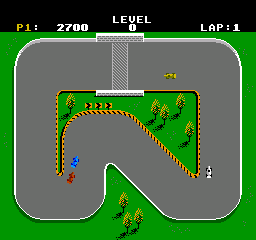
\includegraphics[scale=0.4]{imagenes/super_sprint.png}
        %\end{center}

        \begin{figure}
          \label{logo_latex}
          \begin{center}
            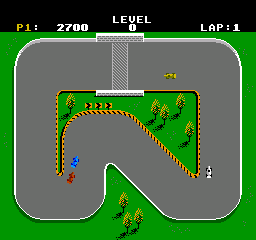
\includegraphics[scale=0.4]{imagenes/super_sprint.png}
          \end{center}
          Super Sprint - Atari (1986)
        \end{figure}
    
        \column{150px}
        \begin{figure}
          \label{logo_latex}
          \begin{center}
            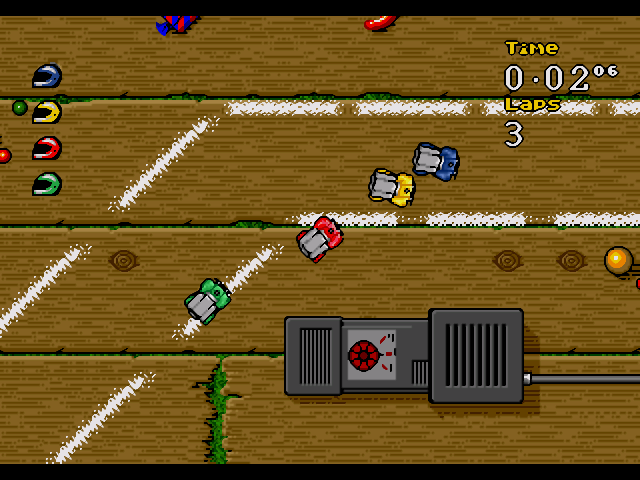
\includegraphics[scale=0.2]{imagenes/micromachines.png}
          \end{center}
          Micromachines - NES (1991)
        \end{figure}

    \end{columns}
    
\end{frame}

\begin{frame}
    \frametitle{Introducción}

    \begin{columns}
    
        \column{150px}
        \begin{block}{Zycars}
            \begin{itemize}
                \item Juego de conducción en 2D con vista cenital
                \item Tres modo de juego
                \item Uso de ítem durante las carreras
            \end{itemize}
        \end{block}

        \column{150px}
        \begin{figure}
          \label{logo_latex}
          \begin{center}
            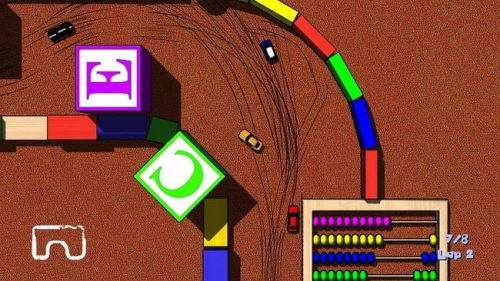
\includegraphics[scale=0.3]{imagenes/toy_cars.jpg}
          \end{center}
          Toy Cars - Xbox 360 (2011)
        \end{figure}
        
    \end{columns}


    \begin{block}{¿Por qué este proyecto?}
        \begin{itemize}
            \item Muy pocos juegos libre con las mismas características
            \item Interés por el mundo de los videojuegos
            \item Cursar la asignatura de Diseño de Videojuegos aumentó el interés por el desarrollo de estos
            \item Contribuir al mundo del software libre
        \end{itemize}
    \end{block}

\end{frame}

\begin{frame}
    \frametitle{Introducción}

    \begin{block}{Objetivos}
        \begin{itemize}
            \item Realizar un juego de coches completamente funcional
            \item Dificultad progresiva (adicción por aprendizaje)
            \item Competidores aceptables, que proponga un desafío superable
            \item Fácilmente ampliable
        \end{itemize}
    \end{block}

    \begin{columns}
    
        \column{200px}
        \begin{alertblock}{No es un simulador}
            \begin{itemize}
                %\item Movimiento básico de los coches
                %\item La colisiones se corrigen de forma sencilla
                \item Arcade, prima la diversión
                \item Coches fáciles de manejar
                \item Colisiones sólo paran a los coches (estrategia)
            \end{itemize}
        \end{alertblock}
        
        \column{100px}
        \begin{figure}
          \label{logo_latex}
          \begin{center}
            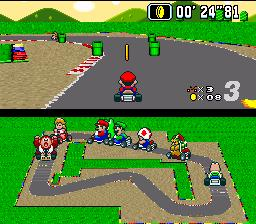
\includegraphics[scale=0.5]{imagenes/super_mario_kart.jpg}
          \end{center}
          Super Mario Kart - SNES (1992)
        \end{figure}
        
    \end{columns}
    
\end{frame}

\clearpage

\chapter{Descripción general del proyecto}

\section{Descripción}

\paragraph{}
El proyecto consiste en un juego de carreras en dos dimensiones con vista cenital, en el que se podrá competirá contra la 
inteligencia artificial. 
La idea es realizar un juego entretenido y dinámico, que estará compuesto por varios modos de juego.

\begin{figure}[H]
  \label{logo_zycars}
  \begin{center}
    
\includegraphics[scale=0.5]{imagenes/logo_zycars.png}
  \end{center}
  \caption{Descripción: Logo de Zycars}
\end{figure}

\section{Características del videojuego}

\paragraph{}
El videojuego ofrece una alternativa libre, gratuita y original para jugar a un juego de conducción en dos dimensiones. 
Las posibilidades que ofrece son las siguientes:

\subsection{Modos de juego}

\paragraph{}
En \emph{Zycars} tendremos distintos modos de juegos, en cada uno de ellos el
objetivo que habrá que llevar a cabo será distinto.
A continuación se describirán los distintos modos de juegos que tendrá el videjuego:

\subsubsection{Carrera rápida} 

\paragraph{}
El juego en el modo de carrera rápida ofrece la posibilidad de enfrentarnos a 3 personajes 
controlados por la inteligencia artificial, a lo largo de un circuito que
hayamos seleccionado previamente. El número de vueltas
que se realicen durante la carrera estarán a elección del jugador y se podrá elegir el número de las mismas a la hora de seleccionar
el circuito.

\subsubsection{Campeonato} 

\paragraph{}
En este modo de juego podremos competir contra 3 personaje controlados por la inteligencia artificial 
a lo largo de un campeonato completo, el cual habremos elegido previamente. 

\paragraph{}
El campeonato estará compuesto por cuatro circuitos y el número de vueltas a estos, también estarán a elección del jugador 
al igual que en el modo de juego explicado anteriormente.

\paragraph{}
Tras la conclusión de cada una de las carreras, los jugadores obtendrán una puntuación en función de la posición que haya 
obtenido. El jugador que mayor puntuación haya conseguido tras acabar los cuatro circuitos, se proclamará ganador del 
campeonato.

\subsubsection{Contrarreloj} 

\paragraph{}
En este último modo de juego y a diferencia de los dos anteriores, el jugador competirá solo sin ningún oponente.

\paragraph{}
El objetivo en este modo de juego será la realización de los circuitos ofrecidos y mejorar los tiempos de estos, ya sean la 
vuelta más rápida del circuito o el tiempo general. El número de vueltas que deberemos dar al circuito serán un total de tres, a
diferencia de los modos anteriores, no tendremos la posibilidad de modificar el valor.

\subsection{Elementos de juego}

\paragraph{}
En esta sección se hará una pequeña descripción de los distintos elementos que encontraremos a lo largo del juego, ya sean 
manipulados por los jugadores, o encontrados a lo largo de los circuitos.

\subsubsection{Personajes}
	
\paragraph{}
Los elementos básico del juego, habrá disponibles distintos personajes que tendrán asociado un 
vehículo característico a su personalidad y apariencia. Cada uno de ellos
tendrán distintas características, 
cosa a tener en cuenta a la hora de hacer nuestra elección por uno de ellos, como la velocidad, la aceleración y el giro.
	
\begin{figure}[H]
	\label{ejemplo_personaje2}
	\begin{center}
		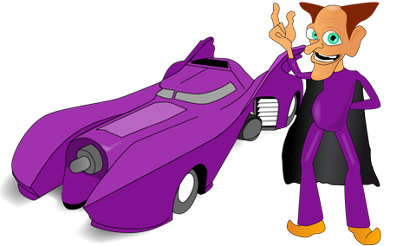
\includegraphics[scale=0.7]{imagenes/ejemplo_personaje2.png}
	\end{center}
	\caption{Descripción: Personaje de Zycars.}
\end{figure}

\subsubsection{Cajas de ítems} 

\paragraph{}
A lo largo de los circuitos en los que estemos compitiendo contra la inteligencia artificial, 
podremos encontrar distintas cajas que al colisionar con ellas nos proporcionen
aleatoriamente una habilidad o ítem que nos
ayuden en la competición contra nuestros rivales.

\begin{figure}[H]
	\label{item_box}
	\begin{center}
		
\includegraphics[scale=1]{imagenes/items/item_box.png}
	\end{center}
	\caption{Descripción: Caja de ítem.}
\end{figure}

\subsubsection{Tipos de ítems}

Los ítems que podremos obtener a partir de la caja de ítems, los podremos diferenciar principalmente en tres tipos:

\begin{description}
	\item \textbf{Ataques a distancia} Estos nos permitirán lanzar ataques
        de forma que podamos interceptar a los competidores que 
	se encuentres lejos de nosotros.
	
	\item \textbf{Obstáculos} Estos nos permitan dejar obstáculos en el
        recorrido, que reduzcan nuestra velocidad considerablemente
	o aquellos que al pasar por encima perdamos completamente el control de nuestro vehículo por unos instantes de tiempo.
	
	\item \textbf{Velocidad} Estos nos darán la opción de aumentar nuestra velocidad durante un pequeño intervalo de tiempo.
\end{description}

\section{Colaboradores}

\paragraph{}
Todo el apartado del proyecto referente a la programación del mismo se ha realizado de forma individual. En cambio, otros apartados
como el diseño gráfico, se ha contado con la colaboración de otra persona, y la música se ha obtenido de internet, concretamente 
de Jamendo, la página de música libre publicadas bajo licencias Creative Commons. Los créditos de juego son los siguientes:

\begin{description}
    \item [Desarrollador] José J. Marente Florín
    \item [Diseñador Gráfico] David Nieto Rojas
    \item [Música] Bob Wizman, Pirato Ketchup, Los Cadaver, The Wavers, Zamalska 
\end{description}

\clearpage

\chapter{Planificación}
\paragraph{}
La planificación realizada para el desarrollo del proyecto, está dividida en varias partes:

%\begin{itemize}
%    \item \textbf{Fase inicial}: la primera fase consistió en plantear la idea del proyecto, con la ayuda del tutor. Tras varias
%    propuestas realizadas y la deliveración sobre las mismas, se decidió realizar este proyecto.
%    
%    \item \textbf{Fase de análisis}: durante esta etapa se realizó la especificación de los requisitos
%    \item \textbf{}:
%    \item \textbf{}:
%    \item \textbf{}:
%    \item \textbf{}:
%\end{itemize}

\section{Fase inicial}

\paragraph{}
La primera fase consistió en plantear la idea del proyecto, con la ayuda del tutor. Tras varias
propuestas y la deliberación sobre las mismas, se decidió realizar este proyecto.

\paragraph{}
También se pensó en que lenguaje se desarrollaría el proyecto, así como las principales bibliotecas
que se usarían durante la realización del mismo.

\section{Fase de análisis}

\paragraph{}
Esta etapa está dividida principalmente en las dos partes siguiente:

\begin{itemize}
    \item \textbf{Especificación de los requisitos}: estudio de los requisitos que deberá cumplir el juego.
    
    \item \textbf{Recurso necesarios}: recursos necesarios que deberemos usar durante el desarrollo del proyecto.
\end{itemize}

\section{Fase Aprendizaje}

\paragraph{}
Dado que el proyecto se realizaría con un lenguaje de programación del que no se tenían conocimientos, en este caso \emph{Python}, 
así como de la biblioteca que usaríamos en el desarrollo, como es \emph{Pygame}, esta fase se dividió en dos partes:

\begin{itemize}
    \item \textbf{Aprendizaje de \emph{Python}}: periodo empleado para el aprendizaje del lenguaje de programación \emph{Python},
    durante esta etapa se consultó varios libros sobre lenguaje, así como foros de internet y páginas web. Para un aprendizaje más
    ameno y llevadero, se realizaron problemas ya resuelto en otros lenguajes.
    
    \item \textbf{Familiarización con la biblioteca \emph{Pygame}}: tras el periodo de aprendizaje del lenguaje, debía familiarizarme
    con la biblioteca principal que se usaría en el desarrollo del proyecto, como es \emph{Pygame}. Durante su
    aprendizaje se realizaron pequeñas aplicaciones sencillas, para asentar
    bien los conocimientos.
\end{itemize}

\section{Fase de desarrollo}

\paragraph{}
Tras la consecución de las etapas anteriores, se comenzó el desarrollo del proyecto. Esta etapa del desarrollo es la más extensa de 
todas, como es comprensible. Y también la etapa que más subetapas contiene, las principales son la siguientes:

\begin{itemize}
    \item \textbf{Motor básico}: implementación de las necesidades básicas del proyecto, como control del teclado, carga de recursos, movimiento
    de los vehículos.
    
    %\item \textbf{Movimiento de vehículos}: relización del movimiento y comportamiento que deberían tener los vehículos: giro, 
    %aceleración, frenada.
    
    \item \textbf{Carga de escenario}: carga de los circuitos que compondrán el juego de forma que no fuera necesario tocar código
    para la ampliación del juego.
    
    \item \textbf{Creación de menús}: implementación de toda la interfaz de menús de la que estaría compuesto el juego, menú de 
    opciones, selección de personaje, selección de circuito, etc.
    
    \item \textbf{Colisiones}: unos de los aspectos más básico y esenciales de cualquier juego, se debía implementar las colisiones con el
    escenario, así como con otros elementos del juego como pueden ser ítems u otros vehículos.
    
    \item \textbf{Ítems}: implementación del comportamiento y efecto que
    producirían cada uno de los ítems que están disponibles en el juego.
    
    \item \textbf{Inteligencia artificial}: planteamiento y desarrollo de los vehículos que serían manejados por la inteligencia 
    artificial, estos deberían de se capaces de evitar obstáculos, realizar
    recorridos y lanzar ítems.
    
    \item \textbf{Modos de juego}: realización de los modos de juego que componen el proyecto, como serían carrera rápida, contrarreloj
    y campeonato,
\end{itemize}

\section{Pruebas y correcciones}

\paragraph{}
Una de las etapas más importantes, si no es la que más, del desarrollo de cualquier proyecto. Esta etapa se realizaría en paralelo
a la de desarrollo, ya que conforme se implementan nuevas funcionalidades, cada
un debía ser probada exhaustivamente en cualquiera
de las posibles situaciones que pudiera suceder.

\section{Redacción de la memoria}

\paragraph{}
La redacción de la memoria se ha realizado conforme se iba avanzando en el desarrollo del proyecto. Pero tras la finalización
del desarrollo se le ha dedicado más tiempo a la realización de esta.

\section{Diagrama de Gantt}

\paragraph{}
A continuación se muestra la planificación anteriormente comentada, en su correspondiente diagrama de Gantt:

\begin{figure}[H]
  \label{gant1}
  \begin{center}
    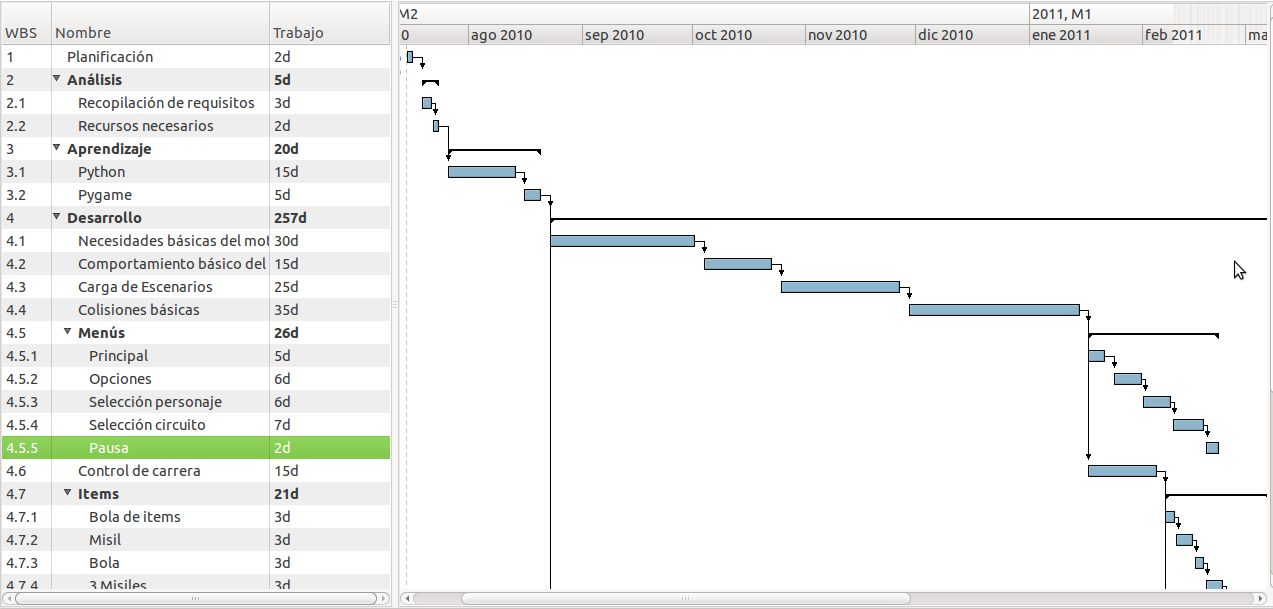
\includegraphics[scale=0.51, angle=90]{imagenes/planificacion/gant1.png}
  \end{center}
  \caption{Planificación: Diagrama de Gantt 1/2.}
\end{figure}

\begin{figure}[H]
  \label{gant2}
  \begin{center}
    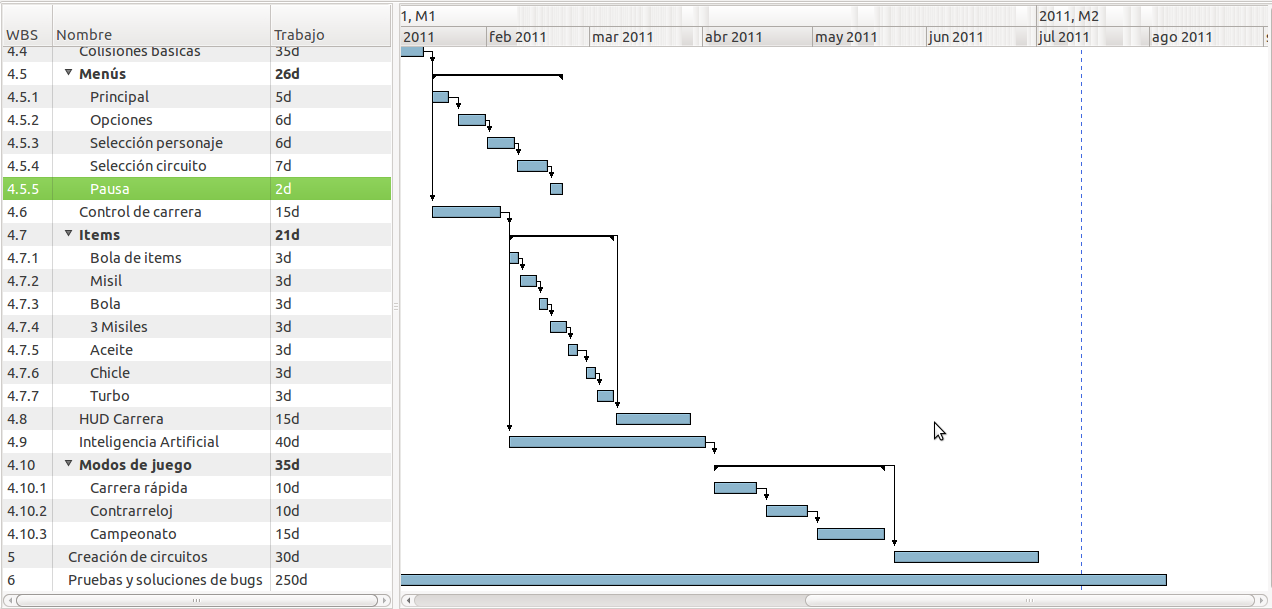
\includegraphics[scale=0.51, angle=90]{imagenes/planificacion/gant2.png}
  \end{center}
  \caption{Planificación: Diagrama de Gantt 2/2.}
\end{figure}

\clearpage

\chapter{Análisis}
%%%%%%%%%%%%%%%%% TOMA DE REQUISITOS %%%%%%%%%%%%%%%%%%%%%%%5
\section{Toma de requisitos}

\paragraph{}
Para la creación de cualquier producto software, es necesario establecer las distintas condiciones y necesidades que
ha de satisfacer. Seguiremos un esquema que nos permita describir los requisitos de una forma metódica y racional.
%\paragraph{}

\subsection{Requisitos de interfaces externas}

\paragraph{}
En este apartado se describirá los requisitos de conexión del software y el hardware, así como la interfaz de usuario.

\paragraph{}
La conexión entres el software y el hardware se encarga la librería \emph{SDL}, mediante el wrapper \emph{Pygame} para 
el lenguaje de programación \emph{Python}. Por lo que al ser un sistema preestablecido, no será necesario realizar el diseño,
ni el análisis, sólo haremos uso de él.

\paragraph{}
Así que pasamos a definir la interfaz entre el usuario y el videojuego. Todas las ventanas de la aplicación tendrán una 
resolución de 800x600 píxeles, siendo posible establecer el modo de pantalla completa \footnote{El modo de pantalla completa
se podrá establecer a través del menú de opciones}. A continuación se distinguen las distintas
ventanas que el usuario encontrará en el sistema:

\begin{description}
    \item \textbf{Ventana de introducción} En esta primera ventana se mostrará únicamente el logotipo del juego, situando al usuario en
    contexto para introducirlo en la ejecución de la aplicación.
    
    \item \textbf{Ventana de menú principal} La ventana del menú principal
    muestra el menú de inicio de \emph{Zycars}, así como 
    todas las opciones generales del juego disponibles, que son las siguientes:
        \begin{itemize}
            \item Carrera Rápida
            \item Campeonato
            \item Contrarreloj
            \item Opciones
            \item Salir
        \end{itemize}
        En este menú y en los siguiente que se describan se usará el ratón para navegar por ellos y solo será necesario
        hacer click sobre la opción deseada para acceder a ella.
    
    \item \textbf{Ventana de opciones} Desde la ventana de opciones se podrán
    modificar las distintas características de la 
    configuración del juego como el audio o controles. Esta ventana se podría dividir en tres partes diferencias que se indican
    a continuación:
        \begin{itemize}
            \item Opciones de audio: podremos modificar el volumen de efectos de sonido y música del juego. También estará la opción
            de silenciar cualquier tipo de sonido.
            
            \item Opciones de pantalla: a través de esta ventana podremos activar o desactivar el modo de pantalla completa.
            
            \item Opciones de control: en esta ventana podremos modificar los controles del juego. Tanto de dirección, lanzamiento
            de ítems y pausa del juego.
        \end{itemize}
    
    \item \textbf{Ventana de selección de personaje} Esta ventana será compartida por los tres modos de juego disponibles. En ella 
    podremos elegir al personaje que desearemos controlar a lo largo de las carreras. De estos jugadores se nos mostrarán sus 
    distintas habilidades.
    
    \item \textbf{Ventana de selección de circuito} Ventana compartida por el modo carrera rápida y contrarreloj. En esta ventana
    deberemos elegir el circuito en el que deseamos competir. Se nos mostrará una imagen de cada circuito que seleccionemos.
    
    \item \textbf{Ventana de selección de campeonato} Ventana muy similar a la descrita anteriormente. En ella se nos mostrarán
    todos los circuitos de cada campeonato disponible. Pero al contrario que la anterior en esta ventana elegiremos el campeonato 
    del circuito seleccionado en el momento.
    
    \item \textbf{Ventana de juego} Ventana principal de todo el juego. Mostrará la carrera actual que se esté disputando, así como
    los distinto marcadores aclaratorios sobre el estado de la carrera, como
    pueden ser posiciones de los jugadores, ítem actual y
    tiempos de carrera. Según la tecla indicada en los controles del menú de opciones (ESC o p) se podrá acceder al menú
    de pausa del juego.
    
    \item \textbf{Ventana de pausa} Únicamente accesible desde la ventana de juego. Esta nos permitirá detener el juego en curso, 
    siendo posible reanudar el juego, reiniciar el mismo o volver al menú principal.
    
    \item \textbf{Ventana de posiciones de carrera} Ventana mostrada al terminar alguna de las carreras. En ella nos muestra el 
    resultado de la última carrera disputada. Nos permite continuar al siguiente circuito, en el caso del modo campeonato, o seguir
    hacia el menú principal, en el modo carrera rápida. También se nos permite
    reiniciar la última carrera disputada.
    
    \item \textbf{Ventana de posiciones de campeonato} Ventana mostrada en el modo campeonato tras la ventana de posiciones 
    de carrera, en ella se nos muestra las posiciones de los competidores en el campeonato actual.
    
    \item \textbf{Ventana de tiempos de contrarreloj} Ventana mostrada al completar algún circuito en el modo contrarreloj. En ella
    se nos muestran los distintos tiempos conseguidos a lo largo del circuito y se nos indicará si hemos batido algún record.
    Esta ventana nos permite continuar hacia el menú principal, así como reiniciar el circuito disputado.
    
\end{description}

\subsection{Requisitos funcionales}

\paragraph{}
Los requisitos funcionales que el sistema debe ofrecer son los siguientes:

\begin{itemize}
    \item Salir de la aplicación desde cualquier ventana.
    \item Seleccionar los distintos modos de juego.
    \item Permitir al jugador competir contra la inteligencia artificial.
    \item Modificar la configuración (audio, pantalla y controles) del juego.
    \item Pausar el juego.
    \item Seleccionar uno de los jugadores propuestos.
    \item Seleccionar cualquiera de los circuitos disponibles.
    \item Seleccionar cualquiera de los campeonatos disponibles.
    \item Reiniciar cualquier carrera una vez terminada o en curso.
    \item Reiniciar cualquier campeonato una vez terminado o en curso.
    \item Lanzamientos de ítems durante cualquier carrera.
\end{itemize}

\paragraph{}
Los distintos tipos de jugadores son:

\begin{itemize}
    \item \textbf{Humano}: es el controlado por una persona
    \item \textbf{Inteligencia artificial}: controlado por el ordenador.
\end{itemize}

\paragraph{}
Existes tres modos de juego:

\begin{itemize}
	\item \textbf{Carrera rápida}: consiste en la realización de un único circuito, compitiendo contra la inteligencia artificial.
	\item \textbf{Campeonato}: el jugador competirá contra la inteligencia artificial a lo largo de 4 carreras, en las que obtendrá una puntuación
	según la posición obtenida en cada una de las carreras. El ganador será el que mejor puntuación haya conseguido al concluir
	el campeonato.
	\item \textbf{Contrarreloj}: en este modo de juego, el jugador competirá solo, con el fin de mejorar las marcas de tiempo de cada uno de los 
	circuitos.
\end{itemize}


\subsection{Requisitos de rendimiento}

\paragraph{}
El rendimiento de la aplicación debe ser tal que permita un desempeño agradable de juego. 

\begin{itemize}
    \item Por lo que la respuesta a las acciones realizadas por el usuario deben ser respondidas lo más rápido posible,
    sacrificando en el caso de que sea necesario el consumo de la memoria principal.
    
    \item La inteligencia artificial debe estar optimizada de forma que no se ralentice la partida en el tiempo dedicado a los
    cálculos necesarios para tomar decisiones.
\end{itemize}
    

\subsection{Restricciones de diseño}

\paragraph{}
Como comento en uno de los puntos del apartado anterior el tiempo de respuesta tiene que primar sobre el consumo de 
memoria principal o secundaria. Esta será la principal restricción de diseño que tendrá nuestra aplicación.

\paragraph{}
Los videojuegos están pensados como aplicación principal, de forma que no tenga que compartir recursos con otros procesos,
por lo que se permitirá que consuma muchos recursos del sistema.

\subsection{Requisitos del sistema software}

\paragraph{}
La aplicación deberá cumplir los siguiente requisitos del sistema:

\begin{itemize}
    \item Deberá ser multiplataforma, al menos en los siguiente sistemas:
    \begin{itemize}
        \item \textbf{Microsoft Windows}: realizando las pruebas sobre la versión Windows 7.
        \item \textbf{GNU/Linux}: usando la distribución Ubuntu 10.10 como principal sistema para pruebas.
    \end{itemize}
    
    \item El código con el que se desarrolle la aplicación no debe ser
    dependiente del sistema en el que se desarrolle.
    
    \item El código debe ser mantenible y fácilmente ampliable para futuras versiones.
\end{itemize}

%%%%%%%%%%%%%%%% MODELO DE CASOS DE USO %%%%%%%%%%%%%%%%%%%%%%%
\section{Modelo de casos de uso}

\paragraph{}
Para describir los distintos comportamientos que tendrá el sistema, usaremos el lenguaje de modelado de sistemas \emph{UML}; que
representa los requisitos funcionales del sistema, centrando en que hace y no cómo lo hace.

\subsection{Diagrama de los casos de uso}

\paragraph{}
En primer lugar mostramos el modelo de casos de uso, que representa la funcionalidad completa de la aplicación. Se ha usado el 
siguiente esquema:

\begin{enumerate}
    \item Identificar los usuarios del sistema y los roles que pueden tener.
    \item Para cada rol, identificar las distintas formas de interactuar en el sistema. En el caso de \emph{Zycars} existe
    un único rol de acceso a la aplicación, por lo que la especificación del usuario será única.
    \item Creación de los casos de uso para todos los objetivos que queramos cumplir.
    \item Estructurar dichos casos de uso.
\end{enumerate}

\begin{figure}[H]
  \label{diagrama_casos_uso}
  \begin{flushleft}
    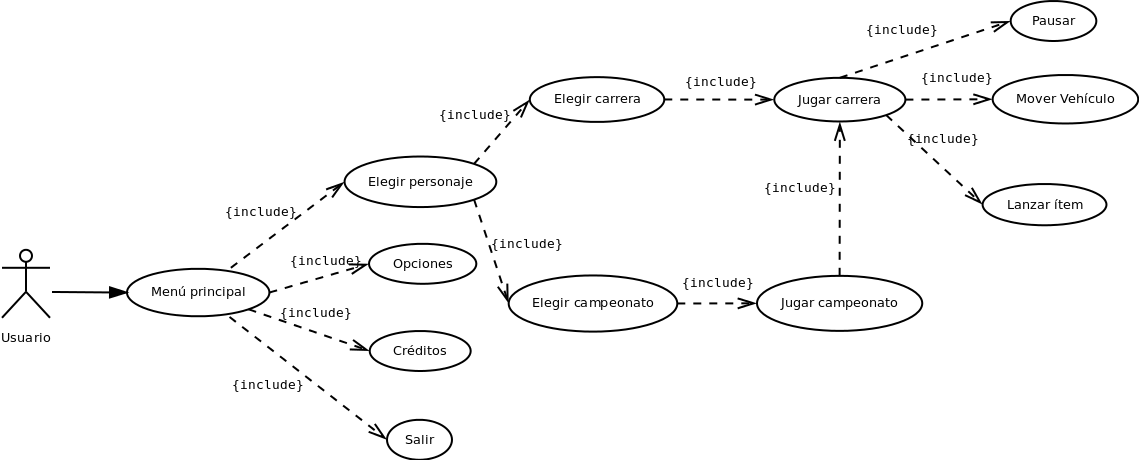
\includegraphics[scale=0.45]{imagenes/analisis/diagrama_casos.png}
  \end{flushleft}
  \caption{Análisis: Diagrama de casos de uso}
\end{figure}

\subsection{Descripción de los casos de uso}

\paragraph{}
A continuación pasamos a la descripción de cada uno de los casos de uso, para la cual usaremos una notación forma usando plantillas.
El texto debe ser legible y comprendido por un usuario que no sea experto.

\subsubsection{Caso de uso: Menú principal}

\begin{description}
    \item[Caso de uso] Menú principal
    \item[Descripción] Se muestra el menú principal de la aplicación, donde es
    posible elegir uno de los modos de juego disponibles
    o acceder al menú de opciones.
    \item[Actores] Usuario
    \item[Precondiciones] Ninguna
    \item[Postcondiciones] Ninguna
    \item[Escenario principal] $\quad$
        \begin{enumerate}
            \item El usuario inicia la aplicación
            \item El sistema muestra el menú principal del juego en pantalla.
            \item El usuario selecciona la opción \textbf{carrera rápida}, \textbf{campeonato} o \textbf{contrarreloj}.
            \item El sistema inicia el modo de elección de personaje.
        \end{enumerate}
    \item[Extensiones --- flujo alternativo] $\quad$
        \begin{description}
            \item[*a ] El usuario cierra la ventana de la aplicación y sale de la aplicación
            
            %\item[2a ] El usuario seleccion la opción \textbf{campeonato}.
            %\begin{enumerate}
            %    \item El sistema inicia el modo de elección de personaje
            %\end{enumerate}
            
            %\item[2b ] El usuario seleccion la opción \textbf{contrarreloj}.
            %\begin{enumerate}
            %    \item El sistema inicia el modo de elección de personaje
            %\end{enumerate}
            
            \item[2a ] El usuario selección la opción \textbf{opciones}.
            \begin{enumerate}
                \item El sistema inicia las opciones
            \end{enumerate}
            
            \item[2b ] El usuario selección la opción \textbf{créditos}.
            \begin{enumerate}
                \item El sistema inicia la opción créditos
            \end{enumerate}
            
            \item[2c ] El usuario selección la opción \textbf{salir}.
            \begin{enumerate}
                \item El sistema sale de la aplicación.
            \end{enumerate}
            
        \end{description}
\end{description}

\subsubsection{Caso de uso: Elegir personaje}

\begin{description}
    \item[Caso de uso] Elegir personaje
    
    \item[Descripción] El usuario desea seleccionar el personaje con el que competirá en el juego, ya sea carrera rápida, 
    campeonato o contrarreloj.
    
    \item[Actores] Usuario
    
    \item[Precondiciones] Ninguna
    
    \item[Postcondiciones] Se selecciona un jugador y se almacenará en la configuración de juego.
    
    \item[Escenario principal] $\quad$
        \begin{enumerate}
            \item El usuario desea seleccionar al personaje que usará en el juego.
            \item El sistema muestra la pantalla de elección de personaje y carga todos los personajes disponibles.
            \item El usuario selecciona un personaje de la lista y pulsa la opción aceptar.
            \item El sistema almacena en la configuración el jugador seleccionado.
            \item El sistema pasa a selección de circuito%, si la precondición es \textbf{carrera rápida} o \textbf{contrarreloj}
        \end{enumerate}
    \item[Extensiones --- flujo alternativo] $\quad$
        \begin{description}
            \item[*a ] El usuario cierra la ventana de la aplicación y sale de la aplicación
            
            \item[*b ] El usuario pulsa la opción cancelar.
            \begin{enumerate}
                \item El sistema vuelve al menú principal
            \end{enumerate}
            
            \item [5a ] El sistema pasa a selección de campeonato.
            
        \end{description}
\end{description}

\subsubsection{Caso de uso: Elegir circuito}

\begin{description}
    \item[Caso de uso] Elegir circuito
    \item[Descripción] El usuario desea seleccionar el circuito en el que desea competir.
    \item[Actores] Usuario
    \item[Precondiciones] El usuario ha elegido previamente en el menú principal una de las opciones: \textbf{carrera rápida} 
    o \textbf{contrarreloj} y ya ha seleccionado un personaje.
    
    \item[Postcondiciones] Se selecciona un circuito y se almacena en la configuración del juego.
    \item[Escenario principal] $\quad$
        \begin{enumerate}
            \item El usuario desea seleccionar el circuito en el que competir.
            \item El sistema muestra todos los circuitos disponibles (icono e imagen) para cada campeonato.
            \item El usuario selecciona un circuito y pulsa aceptar
            \item El sistema almacena el circuito en la configuración del sistema.
            \item El sistema accede a la pantalla de jugar carrera.
        \end{enumerate}
    \item[Extensiones --- flujo alternativo] $\quad$
        \begin{description}
            \item[*a ] El usuario cierra la ventana de la aplicación y sale de la aplicación
            \item[*b ] El usuario pulsa la opción cancelar.
            \begin{enumerate}
                \item El sistema vuelve a la selección de personaje.
            \end{enumerate}
        \end{description}
\end{description}

\subsubsection{Caso de uso: Elegir campeonato}

\begin{description}
    \item[Caso de uso] Elegir campeonato
    \item[Descripción] El usuario desea seleccionar el campeonato que desea realizar.
    \item[Actores] Usuario
    \item[Precondiciones] El usuario ha elegido previamente en el menú principal una de las opciones: \textbf{campeonato} y ha
    elegido un personaje.
    \item[Postcondiciones] Selecciona un campeonato y se almacena en la configuración del juego.
    \item[Escenario principal] $\quad$
        \begin{enumerate}
            \item El usuario desea seleccionar el circuito en el que competir.
            \item El sistema muestra los campeonatos disponibles
            \item El usuario selecciona un campeonato y pulsa sobre la opción aceptar.
            \item El sistema almacena todos los circuitos del campeonato en la configuración del sistema.
            \item El sistema inicia el modo jugar campeonato.
        \end{enumerate}
    \item[Extensiones --- flujo alternativo] $\quad$
        \begin{description}
            \item[*a ] El usuario cierra la ventana de la aplicación y sale de la aplicación
            \item[*b ] El usuario pulsa la opción cancelar.
            \begin{enumerate}
                \item El sistema vuelve a la selección de personaje.
            \end{enumerate}
        \end{description}
\end{description}

\subsubsection{Caso de uso: Jugar carrera}

\begin{description}
    \item[Caso de uso] Jugar carrera
    \item[Descripción] El usuario juega una carrera
    \item[Actores] Usuario
    \item[Precondiciones] El usuario ha seleccionado un circuito o un campeonato.
    \item[Postcondiciones] El usuario completa una carrera.
    \item[Escenario principal] $\quad$
        \begin{enumerate}
            \item El sistema carga el circuito, el jugador, inteligencia artificial y los ítems.
            \item El sistema muestra la pantalla de juego.
            \item El usuario y el sistema interactúan durante la carrera.
            \item El usuario completa la carrera.
            \item El sistema muestra las posiciones finales de la carrera.
            \item El usuario pulsa continuar.
            \item El sistema pasa al menú principal
        \end{enumerate}
    \item[Extensiones --- flujo alternativo] $\quad$
        \begin{description}
            \item[*a ] El usuario cierra la ventana de la aplicación y sale de la aplicación
            %\item[*b] El usuario pulsa el botón de pausa.
             %   \begin{enumerate}
              %      \item El sistema muestra el menú de pausa.
               % \end{enumerate}
        \end{description}
\end{description}

\subsubsection{Caso de uso: Pausar}

\begin{description}
    \item[Caso de uso] Pausar
    \item[Descripción] El usuario selecciona pausar el juego y puede reanudarlo, reiniciarlo o volver al menú principal.
    \item[Actores] Usuario
    \item[Precondiciones] Se está jugando una carrera
    \item[Postcondiciones] Ninguna.
    \item[Escenario principal] $\quad$
        \begin{enumerate}
            \item El usuario pulsa el botón de pausa.
            \item El sistema detiene todos los elementos del juego y muestra el menú de pausa.
            \item El usuario pulsa la opción reanudar.
            \item El sistema reanudar la carrera.
        \end{enumerate}
    \item[Extensiones --- flujo alternativo] $\quad$
        \begin{description}
            \item[*a ] El usuario cierra la ventana de la aplicación y sale de la aplicación

            \item[*b] El usuario pulsa la opción reiniciar.
                \begin{enumerate}
                    \item El sistema reinicia la carrera.
                \end{enumerate}
                
            \item[*b] El usuario pulsa la opción menú.
                \begin{enumerate}
                    \item El sistema vuelve al menú principal.
                \end{enumerate}
        \end{description}
\end{description}

\subsubsection{Caso de uso: Lanzar ítem}

\begin{description}
    \item[Caso de uso] Salir
    \item[Descripción] El usuario lanza el ítem que tenga actualmente.
    \item[Actores] Usuario
    \item[Precondiciones] Se esta jugando una carrera y el usuario a recogido un ítem.
    \item[Postcondiciones] Se añade el ítem a la carrera.
    \item[Escenario principal] $\quad$
        \begin{enumerate}
            \item El usuario pulsa la opción de lanzar ítem.
            \item El sistema comprueba que el usuario posee un ítem y añade el ítem a la carrera.
        \end{enumerate}
    \item[Extensiones --- flujo alternativo] $\quad$
        \begin{description}
            \item[*a ] El usuario cierra la ventana de la aplicación y sale de la aplicación
        \end{description}
\end{description}

\subsubsection{Caso de uso: Mover vehículo}

\begin{description}
    \item[Caso de uso] Mover vehículo
    \item[Descripción] El usuario desplaza al vehículo por el circuito.
    \item[Actores] Usuario
    \item[Precondiciones] Se está jugando una carrera.
    \item[Postcondiciones] Ninguna.
    \item[Escenario principal] $\quad$
        \begin{enumerate}
            \item El usuario pulsa sobre una de las teclas de movimiento. W o Flecha hacia arriba, para mover el vehículo
            hacia adelante o S o Flecha hacia abajo, para moverlo marcha atrás.
            \item El sistema mueve al vehículo teniendo en cuenta su orientación, velocidad y ángulo.
            \item El sistema comprueba que no ha colisionado con ningún obstáculo u otro competidor.
        \end{enumerate}
    \item[Extensiones --- flujo alternativo] $\quad$
        \begin{description}
            \item[*a ] El usuario cierra la ventana de la aplicación y sale de la aplicación
            \item[1a ] El usuario pulsa las teclas de dirección a la vez que avanza. D o Flecha hacia la derecha, para girar
            a la derecha o, A o Flecha hacia la izquierda, para girar a la izquierda.
                \begin{enumerate}
                    \item El sistema gira al coche hacia la zona deseada.
                \end{enumerate}
            \item[3a ] El sistema detecta que ha colisionado con un competidor
            o con algún obstáculo.
                \begin{enumerate}
                    \item El sistema corrige la posición del vehículo.
                \end{enumerate}
        \end{description}
\end{description}

\subsubsection{Caso de uso: Jugar campeonato}

\begin{description}
    \item[Caso de uso] Jugar campeonato
    \item[Descripción] El usuario juega un campeonato.
    \item[Actores] Usuario
    \item[Precondiciones] El usuario selección previamente la opción \textbf{campeonato} en el menú principal.
    \item[Postcondiciones] Se juega un campeonato.
    
    \item[Escenario principal] $\quad$
        \begin{enumerate}
            \item El usuario desea jugar un campeonato
            \item El sistema carga el circuito actual
            \item El sistema y usuario interactúan en la carrera. Include Jugar carrera.
            \item Una vez terminada la carrera el sistema muestras las posiciones del campeonato.
            \item El usuario selección la opción continuar.
            \item El sistema pasar al siguiente circuito.
            \item Volveremos al punto 2.
        \end{enumerate}
    \item[Extensiones --- flujo alternativo] $\quad$
        \begin{description}
            \item[*a ] El usuario cierra la ventana de la aplicación y sale de la aplicación
            
            \item[2a ] Ya no hay más circuitos restantes.
                \begin{enumerate}
                    \item El sistema muestra la clasificación final de todos los jugadores del campeonato.
                    \item El usuario pulsa la opción continuar.
                    \item El sistema muestra la posición del jugador.
                \end{enumerate}
        \end{description}
\end{description}

\subsubsection{Caso de uso: Opciones}

\begin{description}
    \item[Caso de uso] Opciones
    \item[Descripción] El usuario desea modificar las opciones del juego.
    \item[Actores] Usuario
    
    \item[Precondiciones] El usuario seleccionó en el menú principal la opción \textbf{Opciones}.
    \item[Postcondiciones] El usuario modifica las opciones del juego.
    
    \item[Escenario principal] $\quad$
        \begin{enumerate}
            \item El usuario desea modificar las opciones del juego.
            \item El sistema muestra las opciones de juego.
            \item El usuario modifica las distintas opciones de juego.
            \item El usuario esta conforme con los cambios realizados y pulsa sobre el botón aceptar.
            \item El sistema almacena todos los cambios en la configuración.
            \item El sistema vuelve al menú principal.
        \end{enumerate}
    \item[Extensiones --- flujo alternativo] $\quad$
        \begin{description}
            \item[*a ] El usuario cierra la ventana de la aplicación y sale de la aplicación.
            \item[*b ] El usuario selecciona la opción cancelar.
                \begin{enumerate}
                    \item El sistema vuelve al menú principal.
                \end{enumerate}
            
            %\item [4a ] El usuario desea modificar las opciones de pantalla y pulsa sobre el boton de opciones de pantalla.
             %   \begin{enumerate}
              %      \item El sistema muestra las opciones de pantalla.
               %     \item El usuario modifica las distintas opciones de pantalla.
                %\end{enumerate}
            
            %\item [4b ] El usuario desea modificar las opciones de controles y pulsa sobre el boton de opciones de controles.
             %   \begin{enumerate}
              %      \item El sistema muestra las opciones de controles.
               %     \item El usuario modifica las distintas opciones de control.
                %\end{enumerate}
            
        \end{description}
\end{description}

\subsubsection{Caso de uso: Créditos}

\begin{description}
    \item[Caso de uso] Salir
    \item[Descripción] Se muestran la pantalla de créditos donde se reflejan los creadores del juego.
    \item[Actores] Usuario
    \item[Precondiciones] Ninguna.
    \item[Postcondiciones] Ninguna.
    \item[Escenario principal] $\quad$
        \begin{enumerate}
            \item El sistema muestra la pantalla de créditos.
            \item El usuario pulsa la opción volver.
            \item El sistema vuelve al menú principal.
        \end{enumerate}
    \item[Extensiones --- flujo alternativo] $\quad$
        \begin{description}
            \item[*a ] El usuario cierra la ventana de la aplicación y sale de la aplicación
        \end{description}
\end{description}

\subsubsection{Caso de uso: Salir}

\begin{description}
    \item[Caso de uso] Salir
    \item[Descripción] El usuario desea cerrar la aplicación.
    \item[Actores] Usuario
    \item[Precondiciones] Ninguna
    \item[Postcondiciones] Se sale de la aplicación.
    \item[Escenario principal] $\quad$
        \begin{enumerate}
            \item El usuario desea salir de la aplicación.
            \item El usuario pulsa la opción salir del menú principal.
            \item El sistema cierra la aplicación.
        \end{enumerate}
    \item[Extensiones --- flujo alternativo] $\quad$
        \begin{description}
            \item[*a ] El usuario cierra la ventana de la aplicación y sale de la aplicación
        \end{description}
\end{description}

%%%%%%%%%%%%%% MODELO CONCEPTUAL DE DATOS %%%%%%%%%%%%%%%%%%%5
\section{Modelo conceptual de datos}

\paragraph{}
Este apartado del análisis sirve para especificar los requisitos del sistema y las relaciones estáticas que
existen entre ellos.

\paragraph{}
Para este fin se utiliza como herramienta los diagramas de clase. En estos diagramas se representan
las clases de objetos, las asociaciones entre dichas clases, los atributos que componen las clases y las
relaciones de integridad.


\subsection{Diagrama de clases conceptuales}

\paragraph{}
En este apartado se muestra una lista con las diferentes clases necesarias para la realización de sistema. Junto a cada una de
las clases habrá una pequeña descripción sobre la labro que desempeña cada una.

\begin{description}
    \item [Juego] Clase principal de la aplicación, encargada de inicializar el sistema y el flujo entre unos apartados y otros.
    \item [Estado] Clase virtual, con las necesidades básicas de los estados del juego.
    
    \item [Menú Básico] Clase virtual, con las necesidades básicas de los menús.
    \item [Menú principal] Clase que gestiona el menú principal.
    \item [Menú selección personaje] Clase que gestiona el menú de selección de personaje.
    \item [Menú selección circuito] Clase que gestiona el menú de selección de circuito.
    \item [Menú opciones] Clase que gestiona el menú de opciones.
    \item [Menú de pausa] Clase que gestiona el menú de pausa.
    \item [Cursor] Cursor de los menús.
    \item [Botón] Clase que representa el botón en los menús.
    
    \item [Modo de juego] Clase virtual, con las necesidades básicas de los distintos modos de juego.
    \item [Carrera rápida] Clase que gestiona el modo de juego carrera rápida.
    \item [Campeonato] Clase que gestiona el modo de juego campeonato.
    \item [Contrarreloj] Clase que gestiona el modo de juego contrarreloj.
    
    \item [Control de juego] Clase encargada del control de la carrera, controlando la interacción del jugador con el circuito, así 
    como el jugador con la inteligencia artificial. Aspectos básico como colisiones, scroll de pantalla, control de vueltas, control
    de posiciones.
    
    \item [Circuito] Clase encargada de cargar y dibujar el circuito.
    \item [Gestor de colisiones] Clase encargada de detectar y gestionar las colisiones.
    
    \item [Objeto de juego] Clase virtual con las necesidades básicas de los objetos del juego.
    \item [Caja de ítem] Clase que representa las cajas que proporcionan ítems a los jugadores.
    \item [Vehículo básico] Clase virtual con las necesidades básicas de los vehículos del juego.
    \item [IA] Clase que representa el comportamiento de los vehículos controlados por inteligencia artificial.
    \item [Jugador] Clase que que representa al vehículo controlado por el jugador.
\end{description}

\paragraph{}
En las siguientes imágenes podemos ver los diagrama de clases asociado a los requisitos obtenidos. Por razones de espacio en el
documento y para una mejor apreciación de las clases necesarias, se ha visto conveniente dividir en dos partes diferenciadas
principalmente.

\paragraph{}
La primera figura muestra el primer diagrama las clases relacionadas con las pantalla de juego, como pueden ser menús y 
modos de juego.

\begin{figure}[H]
  \label{diagrama_clases_conceptuales}
  \begin{center}
    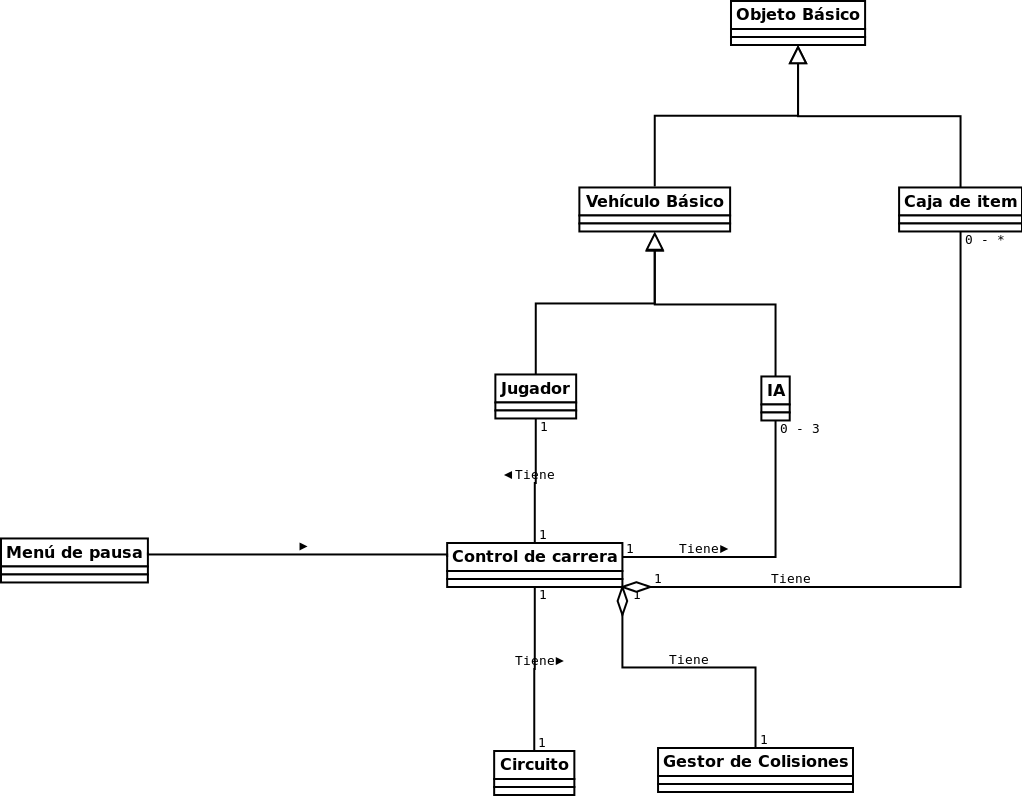
\includegraphics[scale=0.4]{imagenes/analisis/diagrama_clases_conceptuales2.png}
  \end{center}
  \caption{Análisis: Diagrama de clases conceptuales 1}
\end{figure}

\paragraph{}
En la segunda figura vemos el diagrama de clases referente a las clases principales que intervienen en la gestión de la pantalla
de juego.

\begin{figure}[H]
  \label{diagrama_clases_conceptuales}
  \begin{center}
    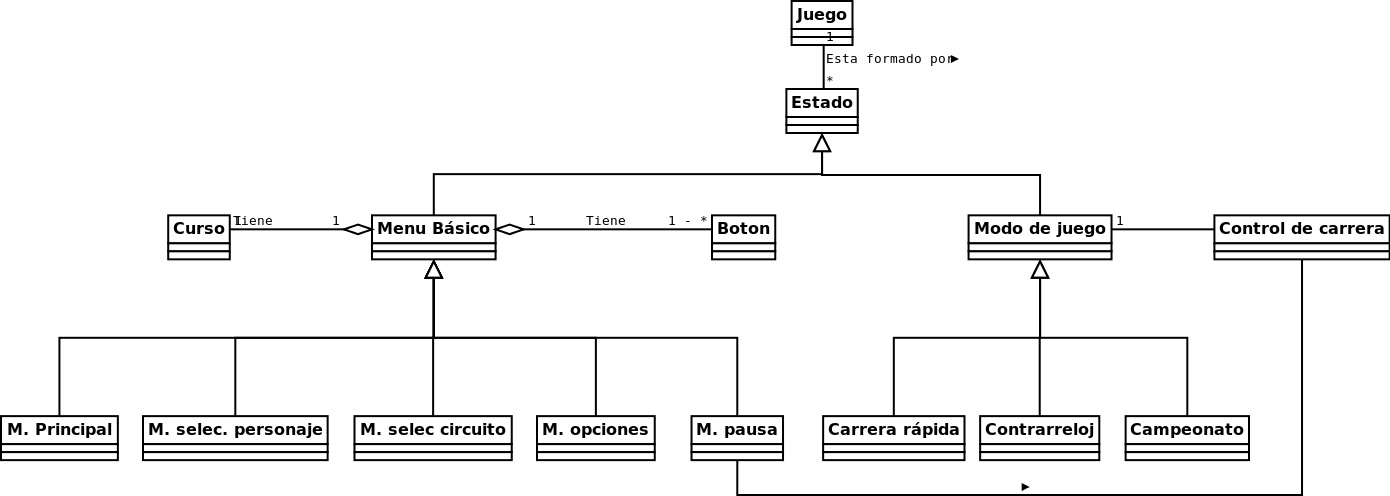
\includegraphics[scale=0.35]{imagenes/analisis/diagrama_clases_conceptuales1.png}
  \end{center}
  \caption{Análisis: Diagrama de clases conceptuales 2}
\end{figure}

\section{Modelo de comportamiento del sistema}

\paragraph{}
El modelo de comportamiento especifica como debe actuar el sistema. El sistema es el que engloba todos los objetos, y el modelo
consta de dos partes:

\begin{itemize}
    \item Diagramas de secuencias del sistema: muestran la secuencia de eventos entre el usuario y el sistema.
    \item Contrato de las operaciones del sistema: describen el efecto que producen las operaciones en el sistema.
\end{itemize}

%%%%%%%%%%%%%%%%%%%%%%%%%%%%%%%%%%%%%%%%%%%%%%%%%%%%%%%%%%%%%%%%%%%%%%%%%%%%%%%%%%%%%%%%%%%%%%%%%%
%%%%%%%%%%%%%%%%%%%%%%%%%%%%%%%%%%%%%%%%%%%%%%%%%%%%%%%%%%%%%%%%%%%%%%%%%%%%%%%%%%%%%%%%%%%%%%%%%%
%%%%%%%%%%%%%%%%%%%%%%%%%%%%%%%%%%%%%%%%%%%%%%%%%%%%%%%%%%%%%%%%%%%%%%%%%%%%%%%%%%%%%%%%%%%%%%%%%%
%%%%%%%%%%%%%%%%%%%%%%%%%%%%%%%%%%%%%%%%%%%%%%%%%%%%%%%%%%%%%%%%%%%%%%%%%%%%%%%%%%%%%%%%%%%%%%%%%%
%%%%%%%%%%%%%%%%%%%%%%%%%%%%%%%%%%%%%%%%%%%%%%%%%%%%%%%%%%%%%%%%%%%%%%%%%%%%%%%%%%%%%%%%%%%%%%%%%%
%%%%%%%%%%%%%%%%%%%%%%%%%%%%%%%%%%%%%%%%%%%%%%%%%%%%%%%%%%%%%%%%%%%%%%%%%%%%%%%%%%%%%%%%%%%%%%%%%%
%%%%%%%%%%%%%%%%%%%%%%%%%%%%%%%%%%%%%%%%%%%%%%%%%%%%%%%%%%%%%%%%%%%%%%%%%%%%%%%%%%%%%%%%%%%%%%%%%%
\subsection{Diagramas de secuencia y contrato de las operaciones del sistema.}

\paragraph{}
No todos los posibles diagramas de secuencia aparecerán, nos centraremos en los más importantes, los que implican algún tipo de 
cambio en el sistema.

\subsubsection{Caso de uso: Menú principal(escenario principal)}

\begin{figure}[H]
  \label{secuencia_menu_principal1}
  \begin{center}
    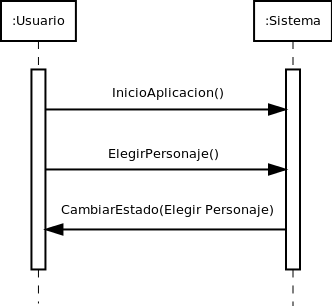
\includegraphics[scale=0.7]{imagenes/analisis/secuencia_menu_principal1.png}
  \end{center}
  \caption{Análisis: Diagrama de secuencia Menú principal (escenario principal)}
\end{figure}

\begin{description}
    \item [Operación] InicioAplicacion()
    \item [Actores] Jugador, sistema.
    \item [Responsabilidades] inicia la aplicación y muestra el menú principal.
    \item [Precondiciones] Ninguna
    \item [Postcondiciones] $\quad$
        \begin{itemize}
            \item El sistema inicia todos los subsistemas necesarios para la correcta ejecución de la aplicación.
            \item El sistema crea un objeto con el Menú principal
        \end{itemize}
\end{description}

\begin{description}
    \item [Operación] ElegirPersonaje()
    \item [Actores] Jugador, Sistema.
    \item [Responsabilidades] salir del menú principal y acceder a la pantalla de elección de personaje.
    \item [Precondiciones] $\quad$
        \begin{itemize}
            \item Existe u objeto del menú principal.
        \end{itemize}
    \item [Postcondiciones] $\quad$
        \begin{itemize}
            \item Se destruye el objeto del menú principal.
        \end{itemize}
\end{description}

\subsubsection{Caso de uso: Menú principal(escenario 2a)}

\begin{figure}[H]
  \label{secuencia_menu_principal2}
  \begin{center}
    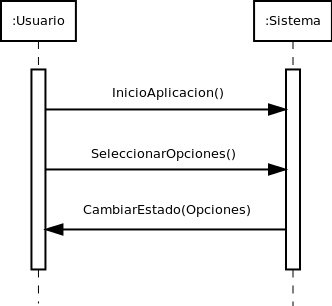
\includegraphics[scale=0.7]{imagenes/analisis/secuencia_menu_principal2.png}
  \end{center}
  \caption{Análisis: Diagrama de secuencia Menú principal (escenario 2a)}
\end{figure}

\begin{description}
    \item [Operación] SeleccionarOpciones()
    \item [Actores] Jugador, Sistema
    \item [Responsabilidades] salir del menú principal y entrar en el menú de opciones.
    \item [Precondiciones] $\quad$
        \begin{itemize}
            \item Existe un objeto del menú principal.
        \end{itemize}
    \item [Postcondiciones] $\quad$
        \begin{itemize}
            \item Se destruye el objeto del menú principal.
        \end{itemize}
\end{description}

\subsubsection{Caso de uso: Menú principal(escenario 2b)}

\begin{figure}[H] 
  \label{secuencia_menu_principal3}
  \begin{center}
    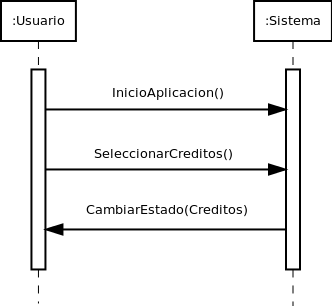
\includegraphics[scale=0.7]{imagenes/analisis/secuencia_menu_principal3.png}
  \end{center}
  \caption{Análisis: Diagrama de secuencia Menú principal (escenario 2b)}
\end{figure}

\begin{description}
    \item [Operación] SeleccionarCréditos()
    \item [Actores] Jugador, sistema.
    \item [Responsabilidades] salir del menú principal y entrar en la pantalla de créditos.
    \item [Precondiciones] $\quad$
        \begin{itemize}
            \item Existe un objeto del menú principal.
        \end{itemize}
    \item [Postcondiciones] $\quad$
        \begin{itemize}
            \item Se destruye el objeto del menú principal.
        \end{itemize}
\end{description}

\subsubsection{Caso de uso: Menú principal(escenario 2c)}

\begin{figure}[H] 
  \label{secuencia_menu_principal4}
  \begin{center}
    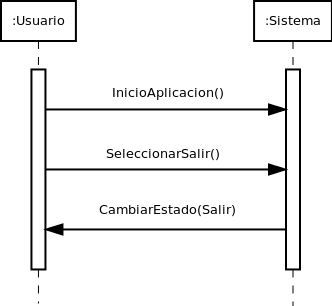
\includegraphics[scale=0.7]{imagenes/analisis/secuencia_menu_principal4.png}
  \end{center}
  \caption{Análisis: Diagrama de secuencia Menú principal (escenario 2c)}
\end{figure}

\begin{description}
    \item [Operación] SeleccionarSalir()
    \item [Actores] Jugador, sistema.
    \item [Responsabilidades] Salir de menú principal y salir de la aplicación
    \item [Precondiciones] $\quad$
        \begin{itemize}
            \item Existe un objeto del menú principal.
        \end{itemize}
    \item [Postcondiciones] $\quad$
        \begin{itemize}
            \item Se destruye el objeto del menú principal.
        \end{itemize}
\end{description}

\subsubsection{Caso de uso: Elegir personaje (escenario principal)}

\begin{figure}[H] 
  \label{secuencia_elegir_personaje}
  \begin{center}
    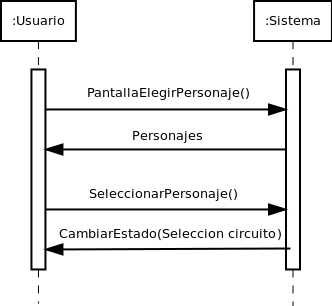
\includegraphics[scale=0.7]{imagenes/analisis/secuencia_elegir_personaje1.png}
  \end{center}
  \caption{Análisis: Diagrama de secuencia Elegir personaje (escenario principal)}
\end{figure}

\begin{description}
    \item [Operación] PantallaElegirPersonaje()
    \item [Actores] Jugador, sistema.
    \item [Responsabilidades] carga y muestra la pantalla de elección de personaje
    \item [Precondiciones] Ninguna
    \item [Postcondiciones] $\quad$
        \begin{itemize}
            \item Crea un objeto de la clase Menú personaje.
        \end{itemize}
\end{description}

\begin{description}
    \item [Operación] SeleccionarPersonaje()
    \item [Actores] Jugador, sistema.
    \item [Responsabilidades] marca un personaje como seleccionado
    \item [Precondiciones] $\quad$
        \begin{itemize}
            \item Existe un objeto del menú de personaje.
            \item Existe el personaje seleccionado.
        \end{itemize}
    \item [Postcondiciones] $\quad$
        \begin{itemize}
            \item Se marca el personaje como seleccionado.
            \item Se destruye el objeto del menú de personaje.
        \end{itemize}
\end{description}

\subsubsection{Caso de uso: Elegir circuito (escenario principal)}

\begin{figure}[H] 
  \label{secuencia_elegir_circuito}
  \begin{center}
    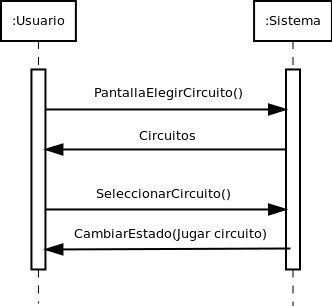
\includegraphics[scale=0.7]{imagenes/analisis/secuencia_elegir_circuito.png}
  \end{center}
  \caption{Análisis: Diagrama de secuencia Elegir circuito (escenario principal)}
\end{figure}

\begin{description}
    \item [Operación] PantallaElegirCircuito()
    \item [Actores] Jugador, sistema.
    \item [Responsabilidades] crea y muestra la pantalla de elección de circuito.
    \item [Precondiciones] Ninguna.
    \item [Postcondiciones] $\quad$
        \begin{itemize}
            \item Crea un objeto de la clase menú de circuito.
        \end{itemize}
\end{description}

\begin{description}
    \item [Operación] SeleccionarCircuito()
    \item [Actores] Jugador, sistema.
    \item [Responsabilidades] marca un circuito como seleccionado.
    \item [Precondiciones] $\quad$
        \begin{itemize}
            \item Existe el circuito seleccionado.
        \end{itemize}
    \item [Postcondiciones] $\quad$
        \begin{itemize}
            \item Se marca el circuito como seleccionado.
            \item Se destruye el objeto de menú de circuito.
        \end{itemize}
\end{description}

\subsubsection{Caso de uso: Elegir campeonato (escenario principal)}

\begin{figure}[H] 
  \label{secuencia_elegir_campeonato}
  \begin{center}
    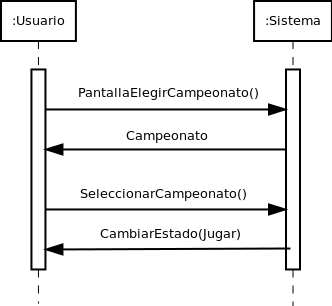
\includegraphics[scale=0.7]{imagenes/analisis/secuencia_elegir_campeonato.png}
  \end{center}
  \caption{Análisis: Diagrama de secuencia Elegir campeonato (escenario principal)}
\end{figure}

\begin{description}
    \item [Operación] PantallaElegirCampeonato()
    \item [Actores] Jugador, sistema.
    \item [Responsabilidades] crea y muestra la pantalla de selección de campeonato
    \item [Precondiciones] Ninguna.
    \item [Postcondiciones] $\quad$
        \begin{itemize}
            \item Crea un objeto de la clase menú campeonato.
        \end{itemize}
\end{description}

\begin{description}
    \item [Operación] SeleccionarCampeonato()
    \item [Actores] Jugador, sistema.
    \item [Responsabilidades] selecciona un campeonato.
    \item [Precondiciones] $\quad$
        \begin{itemize}
            \item Existe el campeonato seleccionado.
        \end{itemize}
    \item [Postcondiciones] $\quad$
        \begin{itemize}
            \item Se marca el campeonato seleccionado.
            \item Se destruye el objeto de menú campeonato.
        \end{itemize}
\end{description}

\subsubsection{Caso de uso: Jugar carrera (escenario principal)}

\begin{figure}[H] 
  \label{secuencia_jugar}
  \begin{center}
    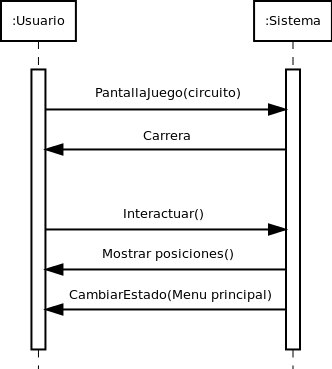
\includegraphics[scale=0.7]{imagenes/analisis/secuencia_jugar.png}
  \end{center}
  \caption{Análisis: Diagrama de secuencia Jugar carrera (escenario principal)}
\end{figure}

\begin{description} 
    \item [Operación] PantallaJuego()
    \item [Actores] Jugador, sistema.
    \item [Responsabilidades] carga y muestra la pantalla de jugo con el circuito seleccionado, inicia el juego.
    \item [Precondiciones] Ninguna
    \item [Postcondiciones] $\quad$
        \begin{itemize}
            \item Se crea un objeto de Control de juego.
            \item Se crea un objeto de Circuito
            \item Se crea un objeto de Jugador.
            \item Se crea un objeto de Gestor de colisiones.
            \item Se crea un objeto de IA por cada competidor de carrera.
            \item Se crea un objeto de Caja de ítem por cada caja del circuito.
        \end{itemize}
\end{description}

\begin{description}
    \item [Operación] Interactuar()
    \item [Actores] Jugador, sistema.
    \item [Responsabilidades] permite al jugador interactuar con el mundo 2D y los elementos que este posee.
    \item [Precondiciones] $\quad$
        \begin{itemize}
            \item Existe un objeto de Control de juego.
            \item Existe un objeto de Jugador.
        \end{itemize}
    \item [Postcondiciones] Ninguna.
\end{description}

\subsubsection{Caso de uso: Pausar (escenario principal)}

\begin{figure}[H] 
  \label{secuencia_pausar1}
  \begin{center}
    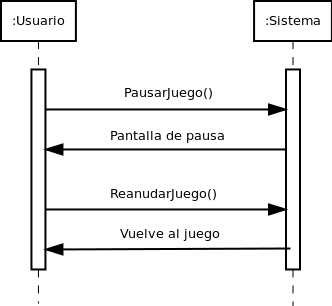
\includegraphics[scale=0.7]{imagenes/analisis/secuencia_pausar1.png}
  \end{center}
  \caption{Análisis: Diagrama de secuencia Pausar(escenario principal)}
\end{figure}

\begin{description}
    \item [Operación] PausarJuego()
    \item [Actores] Jugador, sistema.
    \item [Responsabilidades] pausa el juego y detiene todos los elementos de este.
    \item [Precondiciones] $\quad$
        \begin{itemize}
            \item Existe un objeto de Control juego.
            \item Se está jugando una carrera.
        \end{itemize}
    \item [Postcondiciones]
        \begin{itemize}
            \item Se crea un objeto de Menú de pausa.
        \end{itemize}
\end{description}

\begin{description}
    \item [Operación] ReanudarJuego()
    \item [Actores] Jugador, sistema.
    \item [Responsabilidades] reanuda la partida y quita el menú de pausa.
    \item [Precondiciones] $\quad$
        \begin{itemize}
            \item Existe un objeto de Control juego.
            \item La carrera estaba pausada
        \end{itemize}
    \item [Postcondiciones] $\quad$
        \begin{itemize}
            \item Se destruye el objeto del menú de pausa.
        \end{itemize}
\end{description}

\subsubsection{Caso de uso: Pausar (escenario *b)}

\begin{figure}[H] 
  \label{secuencia_pausar2}
  \begin{center}
    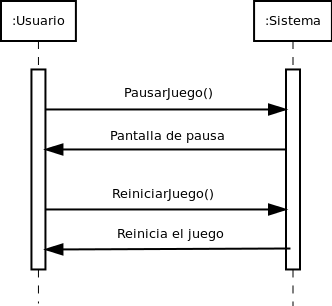
\includegraphics[scale=0.7]{imagenes/analisis/secuencia_pausar2.png}
  \end{center}
  \caption{Análisis: Diagrama de secuencia Pausar (escenario *b)}
\end{figure}

\begin{description}
    \item [Operación] ReiniciarJuego()
    \item [Actores] Jugador, sistema.
    \item [Responsabilidades] reinicia la carrera que se estaba jugando.
    \item [Precondiciones] $\quad$
        \begin{itemize}
            \item Existe un objeto de Control juego.
            \item La carrera estaba pausada
        \end{itemize}
    \item [Postcondiciones] $\quad$
        \begin{itemize}
            \item Se destruye el objeto del menú de pausa.
            \item Se reinicia la carrera.
        \end{itemize}
\end{description}

\subsubsection{Caso de uso: Pausar (escenario *c)}

\begin{figure}[H] 
  \label{secuencia_pausar3}
  \begin{center}
    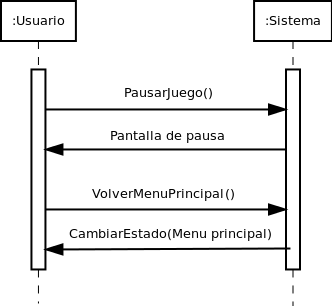
\includegraphics[scale=0.7]{imagenes/analisis/secuencia_pausar3.png}
  \end{center}
  \caption{Análisis: Diagrama de secuencia (escenario )}
\end{figure}

\begin{description}
    \item [Operación] VolverMenuPrincipal()
    \item [Actores] Jugador, sistema.
    \item [Responsabilidades] se para la carrera jugada y se vuelve al menú principal.
    \item [Precondiciones] $\quad$
        \begin{itemize}
            \item Existe un objeto de Control juego.
            \item La carrera estaba pausada
        \end{itemize}
    \item [Postcondiciones] $\quad$
        \begin{itemize}
            \item Se destruye el objeto del menú de pausa.
        \end{itemize}
\end{description}

\subsubsection{Caso de uso: Lanzar ítem (escenario principal)}

\begin{figure}[H] 
  \label{secuencia_lanzar_item}
  \begin{center}
    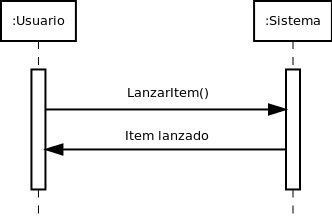
\includegraphics[scale=0.7]{imagenes/analisis/secuencia_lanzar_item.png}
  \end{center}
  \caption{Análisis: Diagrama de secuencia Lanzar ítem (escenario principal)}
\end{figure}

\begin{description}
    \item [Operación] LanzarItem()
    \item [Actores] Jugador, sistema.
    \item [Responsabilidades] hace que el jugador lance el ítem que tiene en ese momento.
    \item [Precondiciones] $\quad$
        \begin{itemize}
            \item Existe un objeto de Control juego.
            \item Existe un objeto de jugador.
            \item El jugador posee un ítem.
        \end{itemize}
    \item [Postcondiciones] $\quad$
        \begin{itemize}
            \item Se crea un objeto ítem.
            \item Se añade el objeto ítem a Control de juego.
        \end{itemize}
\end{description}

\subsubsection{Caso de uso: Mover vehículo (escenario principal)}

\begin{figure}[H] 
  \label{secuencia_mover_vehiculo}
  \begin{center}
    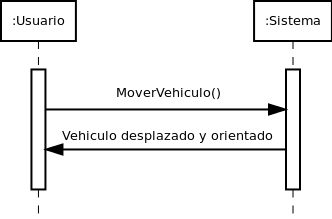
\includegraphics[scale=0.7]{imagenes/analisis/secuencia_mover_vehiculo.png}
  \end{center}
  \caption{Análisis: Diagrama de secuencia Mover vehículo (escenario principal)}
\end{figure}

\begin{description}
    \item [Operación] MoverVehiculo()
    \item [Actores] Jugador, sistema.
    \item [Responsabilidades] mueve al personaje por el mundo 2D.
    \item [Precondiciones] $\quad$
        \begin{itemize}
            \item Existe un objeto de Control juego.
            \item Existe un objeto de jugador.        
        \end{itemize}
    \item [Postcondiciones] $\quad$
        \begin{itemize}
            \item Se modifica la posición del objeto jugador.
        \end{itemize}
\end{description}

\subsubsection{Caso de uso: Opciones (escenario principal)}

\begin{figure}[H] 
  \label{secuencia_opciones}
  \begin{center}
    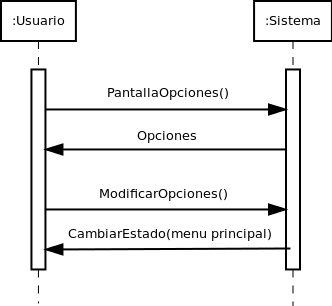
\includegraphics[scale=0.7]{imagenes/analisis/secuencia_opciones.png}
  \end{center}
  \caption{Análisis: Diagrama de secuencia opciones (escenario principal)}
\end{figure}

\begin{description}
    \item [Operación] PantallaOpciones()
    \item [Actores] Jugador, sistema.
    \item [Responsabilidades] se crea y muestra la pantalla de opciones.
    \item [Precondiciones] Ninguna.
    \item [Postcondiciones] $\quad$
        \begin{itemize}
            \item Se crea un objeto de menú de opciones
        \end{itemize}
\end{description}

\begin{description}
    \item [Operación] ModificarOpciones
    \item [Actores] Jugador, sistema.
    \item [Responsabilidades] se modifican las opciones y se vuelve al menú principal.
    \item [Precondiciones] $\quad$
        \begin{itemize}
            \item Existe un objeto de menú de opciones
        \end{itemize}
    \item [Postcondiciones] $\quad$
        \begin{itemize}
            \item Se aplican los cambios de opciones.
            \item Se destruye el objeto de menú de opciones.
        \end{itemize}
\end{description}

\subsubsection{Caso de uso: Créditos (escenario principal)}

\begin{figure}[H] 
  \label{secuencia_creditos}
  \begin{center}
    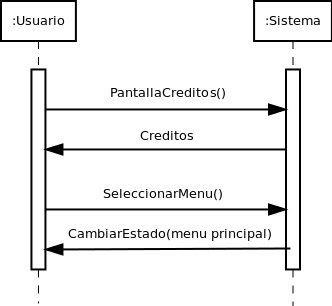
\includegraphics[scale=0.7]{imagenes/analisis/secuencia_creditos.png}
  \end{center}
  \caption{Análisis: Diagrama de secuencia Créditos(escenario principal)}
\end{figure}

\begin{description}
    \item [Operación] PantallaCréditos()
    \item [Actores] Jugador, sistema.
    \item [Responsabilidades] crea y muestra la pantalla de créditos
    \item [Precondiciones] Ninguna.
    \item [Postcondiciones] $\quad$
        \begin{itemize}
            \item Se crea un objeto de Menú de créditos.
        \end{itemize}
\end{description}

\begin{description}
    \item [Operación] SeleccionarMenu()
    \item [Actores] Jugador, sistema.
    \item [Responsabilidades] destruye la pantalla de créditos y vuelve el menú principal.
    \item [Precondiciones] $\quad$
        \begin{itemize}
            \item Existe un objeto de Menú de créditos.
        \end{itemize}
    \item [Postcondiciones] $\quad$
        \begin{itemize}
            \item Se destruye el objeto de Menú de créditos.
        \end{itemize}
\end{description}

\clearpage

\chapter{Diseño}

%En primer lugar para describir el diseño de la aplicación se describirán los requisitos del sistema
%necesarios para la ejecución de la aplicación, posteriormente comentaremos que herramientas se va usar a lo largo
%del desarrollo.

\paragraph{}
Al igual que en el apartado referente al análisis del sistema, en el diseño de este también usaremos una metodología orientada
a objetos mediante UML.

\paragraph{}
Este proceso es mucho mas sencillo una vez que ya se ha especificado que hace el sistema en el capítulo anterior. También decir, que
al igual que el análisis del sistema, el diseño no contempla muchos detalles del sistema final, sólo una idea orientativa de como
se implementará el sistema.

\paragraph{}
En este capítulo no se han añadido descripciones de las clases que componen el sistema, para ello se encuentra disponible toda la
documentación del código, donde esta toda la información necesaria referente a las clases y archivos que componen la aplicación.

\section{Interfaz gráfica}

\paragraph{}
Tras los resultado que se han obtenido en la fase de analisis del sistema, es necesario desarrolar una interfaz sencilla y agradable
para el usuario de la misma. En el diseño de estos, se intentará en todo momento que el usuario no tenga la posibilidad de insertar
datos erroneos que lleven a una ejecución anómala de la aplicación.

\begin{figure}[H]
  \label{interfaz}
  \begin{center}
    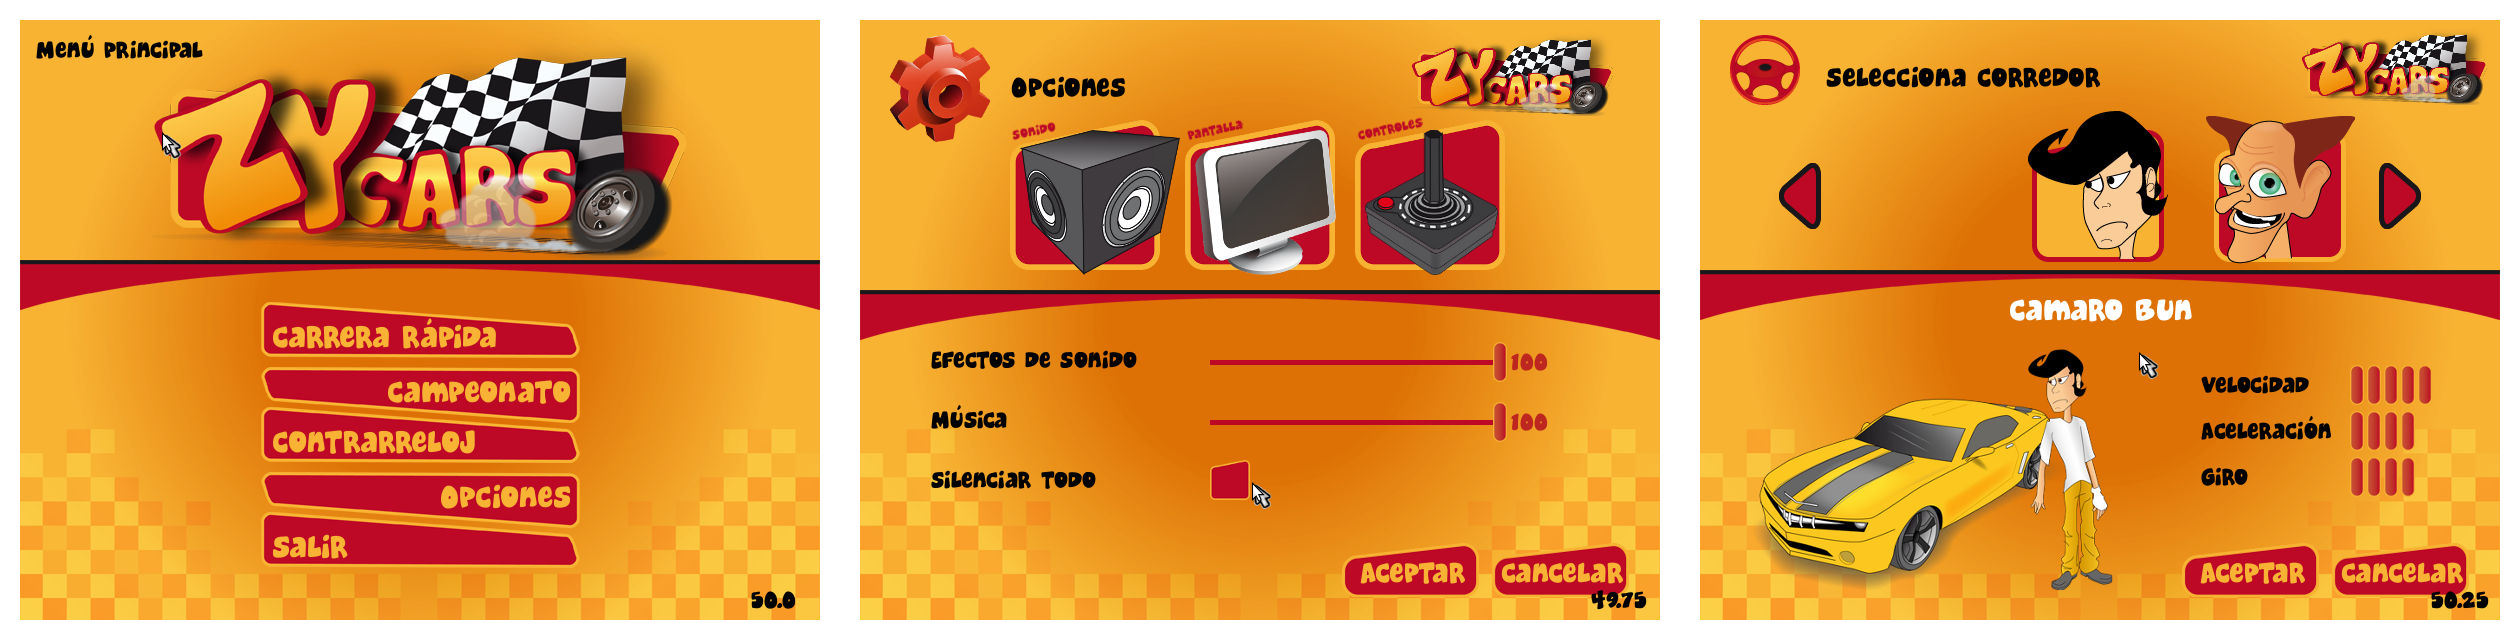
\includegraphics[scale=0.18]{imagenes/capturas/interfaz.png}
  \end{center}
  \caption{Diseño: Capturas de la interfaz del sistema}
\end{figure}

\subsection{Diagrama de interacción entre interfaces}

\paragraph{}
En la imagen que se muestra a continuación podemos observar la interacción entre las distintas interfaces graficas que se han 
desarrollado para la aplicación.

\begin{figure}[H]
  \label{diagrama_interaccion}
  \begin{center}
    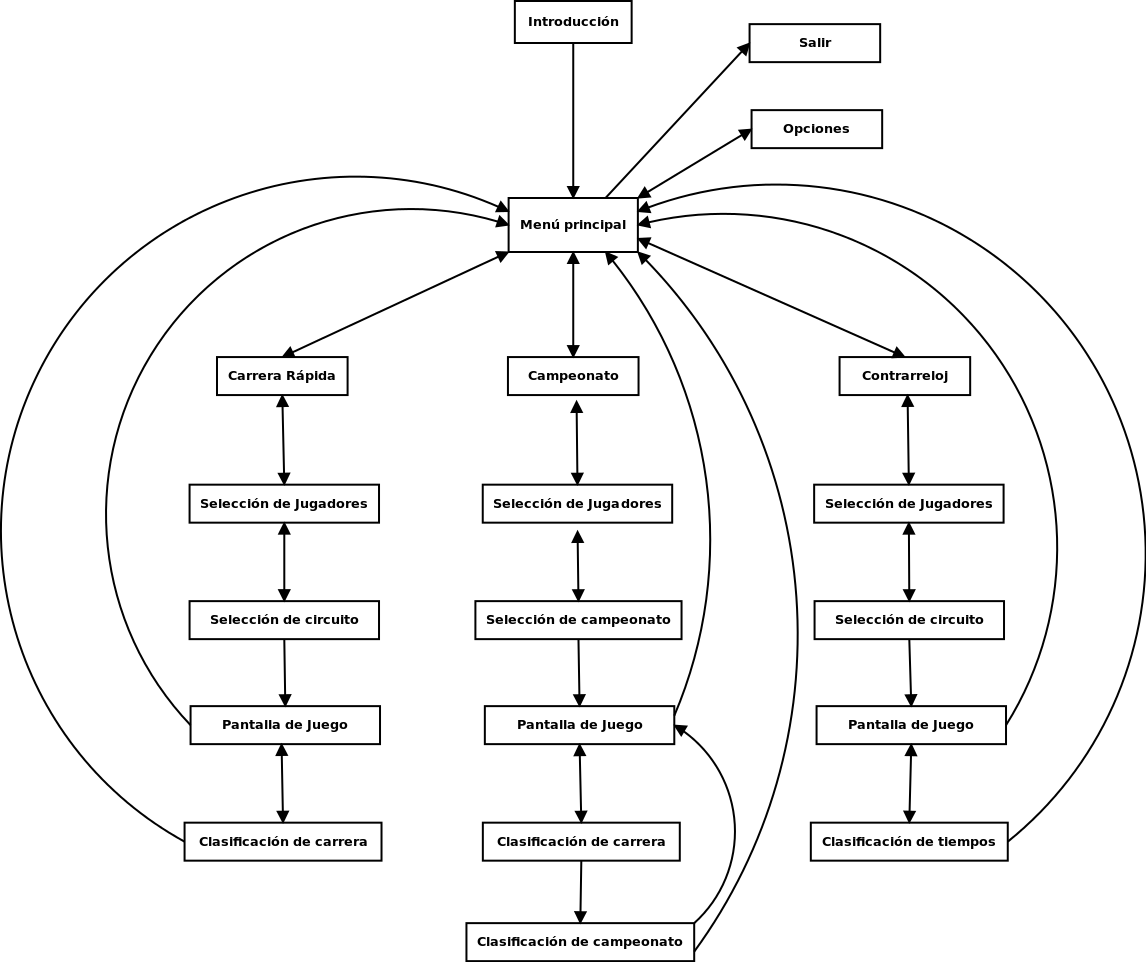
\includegraphics[scale=0.4]{imagenes/diseno/diagrama_interaccion.png}
  \end{center}
  \caption{Diseño: Diagrama de interacción}
\end{figure}

\section{Diagrama de clases de diseño}

A continuación se presenta el diagrama de clases de diseño de \emph{Zycars}.

\newpage

\begin{figure}[H]
  \label{diagrama_clases_diseno}
  \begin{center}
    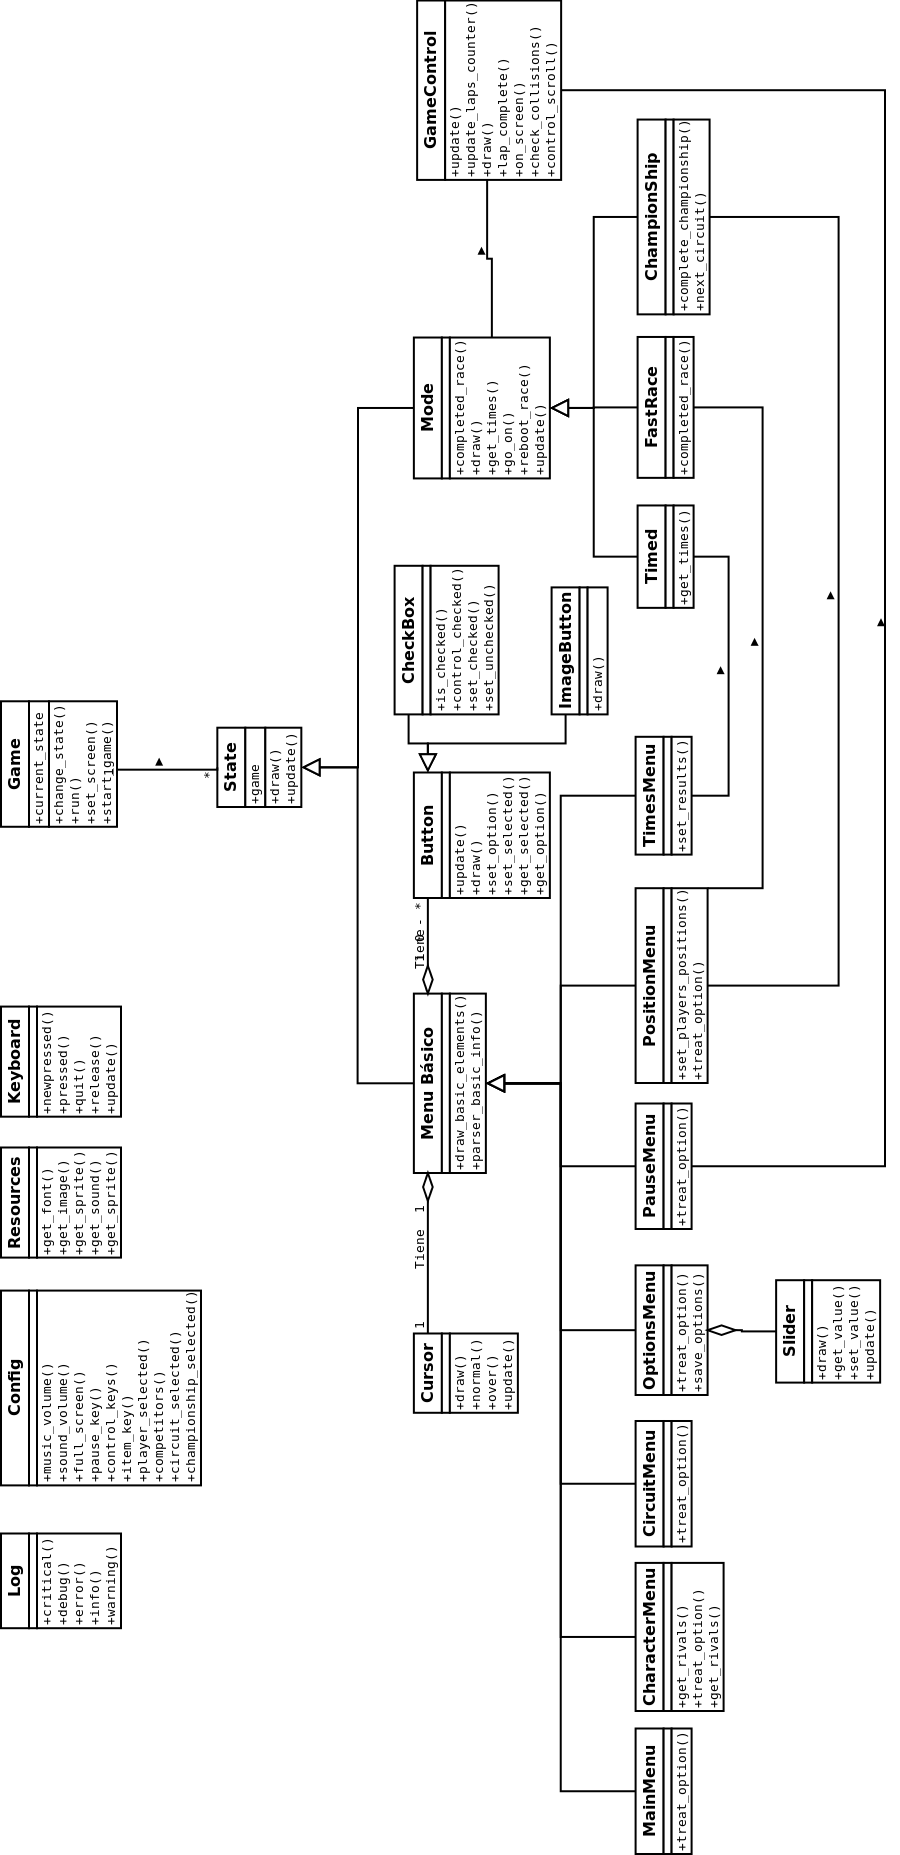
\includegraphics[scale=0.38]{imagenes/diseno/diagrama_clases_diseno1.png}
  \end{center}
  \caption{Diseño: Diagrama de clases de diseño 1}
\end{figure}

\begin{figure}[H]
  \label{diagrama_clases_diseno}
  \begin{center}
    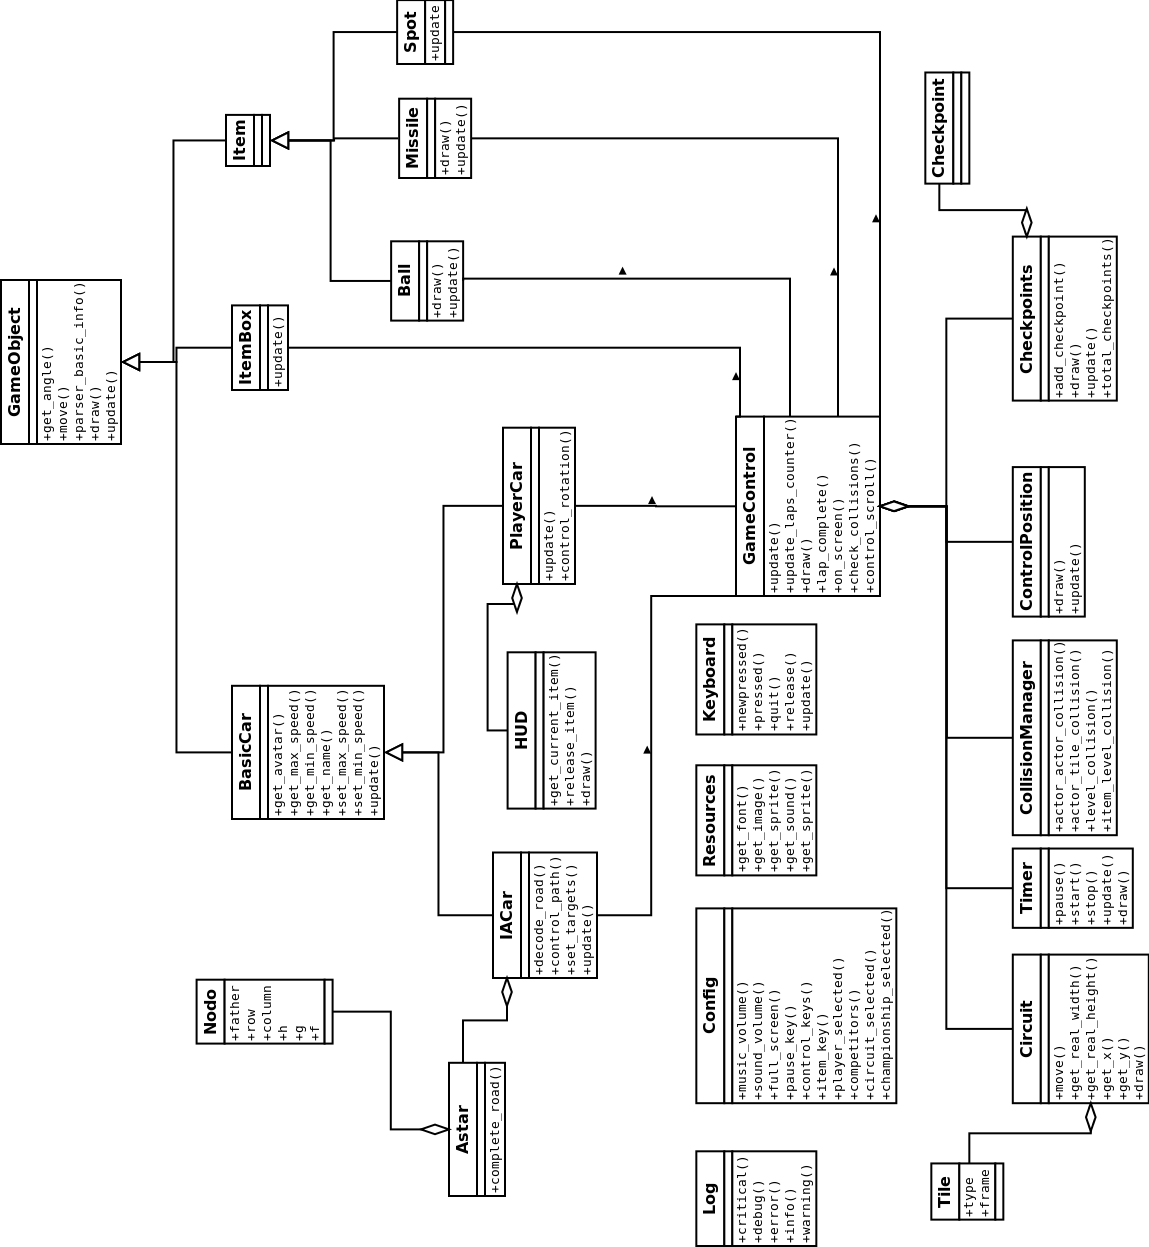
\includegraphics[scale=0.45]{imagenes/diseno/diagrama_clases_diseno2.png}
  \end{center}
  \caption{Diseño: Diagrama de clases de diseño 2}
\end{figure}

\section{Diagramas de secuencia}
lalalal

\clearpage

\chapter{Implementación}
\begin{frame}
    \frametitle{Separar datos del código}

        En todo momento se ha procurado separar todos los datos de los personajes, circuitos y menús, del código
        fuente.\\
        \begin{block}{Ventajas}
            \begin{itemize}
                \item No es necesario saber programar para realizar cambios sobre cualquier parámetro.
                \item Cualquier persona puede ampliar el juego con nuevos personajes y nuevos circuitos, siguiendo
                los manuales creados para ello.
            \end{itemize}
        \end{block}
        \begin{block}{Solución}
            \begin{itemize}
                \item Todo se lee de ficheros XML
            \end{itemize}
        \end{block}

\end{frame}

\begin{frame}
    \frametitle{Formato de circuitos}

    \begin{block}{Mapas de tiles}
        Tile: imagen cuadrada, rectangular o hexagonal, utilizada para generar imágenes de mayor complejidad.
    \end{block}   
    
    \begin{block}{Editor de mapas: Tiled}
    Proporcionaba todas las necesidades básicas, 
    como una sencilla edición y creación de niveles, así como la gestión de capas,
    para poder poner elementos en el circuito a un nivel superior o inferior.\\
    Para ello se debía crear una imagen con todos los tiles que compondrían un circuito (tileset).\\
    Genera como resultado un XML.
    \end{block}   

    \begin{block}{Inconveniente}
        No permitia indicar de forma sencilla que tiles eran atravesables, colisionables o de cualquier otro tipo.
    \end{block}

\end{frame}

\begin{frame}
    \frametitle{Formato de circuitos}

        \begin{block}{Solución}
        Una imagen extra con las mismas características, donde los tiles sera de un único color, en función del tipo
        que estos sean.
        \end{block}

        \begin{center}
                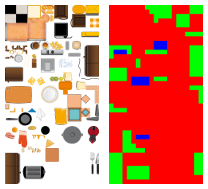
\includegraphics[scale=0.15]{imagenes/tileset-collisionmap.png}
        \end{center}
        

\end{frame}

\begin{frame}
    \frametitle{Colisiones}
    
    Una de las cosas más básicas en cualquier tipo de juego.

    \begin{block}{Colisión con el escenario}
        \begin{itemize}
            \item Detectamos si atravesamos algún tile no atravesable
            \item Si es así corregimos la posición del coche en según la dirección, sentido y lado del tile por
            el que colisione
            \item En el caso de que el tile sea de tipo realentizador, diminuimos la velocidad del coche
        \end{itemize}
    \end{block}

    \begin{center}
        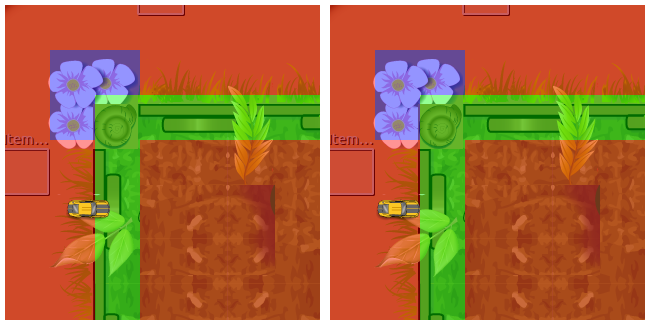
\includegraphics[scale=0.3]{imagenes/colision1-colision2.png}
    \end{center}
\end{frame}

\begin{frame}
    \frametitle{Colisiones}
    
    \begin{block}{Colisión entre vehículos}
        \begin{itemize}
            \item De forma similar a la colisión con el escenario
            \item Cuando se detecta la colisión se corrige la posición de los vehículos, en función la dirección, 
            sentido y lado del tile por el que colisionen
        \end{itemize}
    \end{block}
    
    \begin{block}{Colisión entre vehículos e ítems}
        \begin{itemize}
            \item Si es un ítem de ataque a distancia, destruiremos dicho ítem y cambiaremos el estado del coche con el que
            colisione
            \item Si el ítem es un obstaculo, cambiaremos el estado del coche en función del tipo de ítem
        \end{itemize}
    \end{block}

\end{frame}

\begin{frame}
    \frametitle{Inteligencia artificial}
    Otro de los aspectos más importante de un videojuego de las características de Zycars, es la
    inteligencia artificial, ya que en dos de los tres modos de juegos disponibles el objetivo es obtener la
    mejor clasificación posible, por delante de los demás coches controlados por el ordenador

        \begin{block}{Habilidades}
            \begin{itemize}
                \item Realización del recorrido: debe ser capaz de realizar los 
                recorridos de los circuitos.
                \item Lanzamiento de ítems: también debe poder usar los ítems que reciba de las bolas de ítems.
            \end{itemize}
        \end{block}
\end{frame}

\begin{frame}
    \frametitle{Realización del recorrido. Algoritmo A*}

    Aprovechando que tenemos un circuito creado por tiles y que podemos saber en todo momento en el tile 
    actual que se puede encontrar cualquiera de los competidores, se decidió implementar el 
    algoritmo de búsqueda A*.

        \begin{block}{Objetivo}
        Buscar el camino más corto y óptimo, en el caso de que exista, desde
        un nodo origen, hasta un nodo destino. A la hora de buscar dicho camino se tienen en cuenta factores
        como, el valor heurístico que poseen cada uno de los nodos, así como el coste real del recorrido.
        \end{block}

        \begin{block}{Parámetros}
        Los parametros que se tienen en cuenta en cada uno de los nodos.
            \begin{itemize}
                \item h’(n) es el valor heurístico del nodo actual n, hasta el final
                \item g(n) el coste real del camino desde el origen al nodo actual
                \item Función de evaluación: f(n) = g(n) + h’(n)
            \end{itemize}
        \end{block}

\end{frame}

\begin{frame}
    \frametitle{Realización del recorrido. Algoritmo A*}

        \begin{block}{Estructuras diferenciadas}
            \begin{itemize}
                \item Lista de abiertos: nodos por los que aún no se han pasado
                \item Lista de cerrados: nodos por los que ya se han pasado
            \end{itemize}
        \end{block}

        \begin{block}{Funcionamiento}
            Partiendo de un nodo en el que nos encontramos actualmente:
            \begin{enumerate}
                \item Obtenemos vecinos
                \item Comprobamos que no esten en abiertos ni cerrados
                \item Si alguno esta en abiertos, comprobamos su f(n), si es menor lo sustituiremos
                \item Introducimos en abiertos los que cumplan las condiciones
                \item Obtener de abiertos el nodo que tenga un f(n) menor y comenzamos de nuevo todo el proceso.
                \item Una vez lleguemos al nodo objetivo, detenemos la búsqueda y devolvemos el camino completo.
            \end{enumerate}
        \end{block}

\end{frame}

\begin{frame}
    \frametitle{Realización del recorrido. Algoritmo A*}

        Aplicación en Zycars

        \begin{center}
                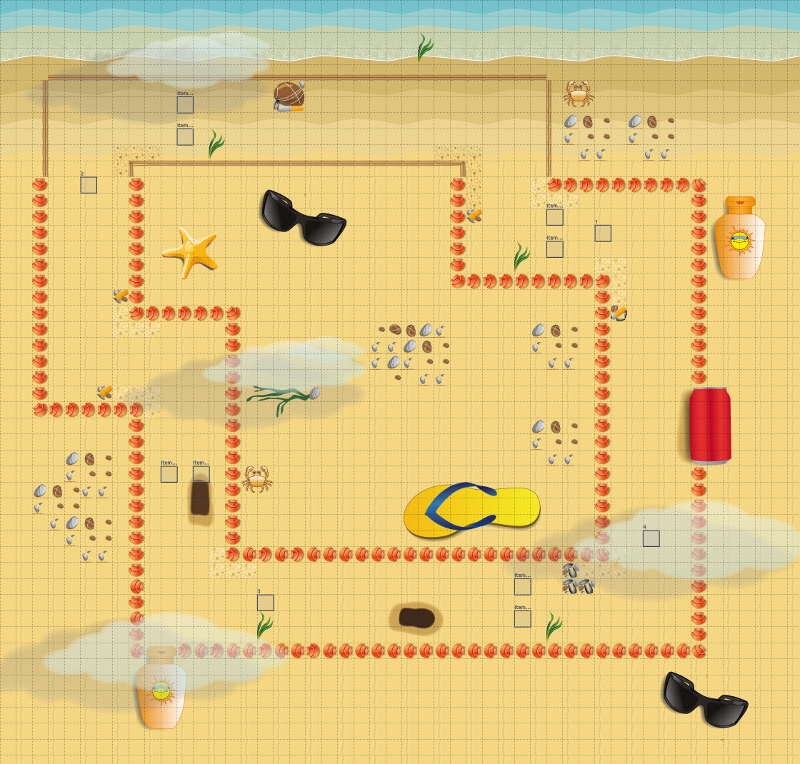
\includegraphics[scale=0.3]{imagenes/ia_check.png}
        \end{center}
        
\end{frame}

\begin{frame}
    \frametitle{Lanzamientos de ítems}

    Capaz de lanzar los ítems disponibles a los largo del juego, según las
    distintas situaciones en la que se encuentre.

        \begin{block}{Solución}
        Se eligió una forma muy sencilla y eficiente a la hora de realizarlo. Para ello cada
        vehículo controlado por la inteligencia artificial, tiene tanto un segmento que va desde el centro del
        coche hacia unos píxeles por delante de la posición actual del vehículo, como otro segmento que
        también va desde el centro pero uno píxeles atrás de la posición del vehículo.
        \end{block}

        \begin{center}
                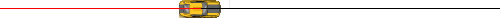
\includegraphics[scale=0.5]{imagenes/ia_segmentos.png}
        \end{center}

\end{frame}

\clearpage

\chapter{Pruebas}

\paragraph{}
El diseño de casos de pruebas para un videojuego es algo complicado, no sólo para \emph{Zyars}, si no para la mayoría de los
distintos tipos de videojuegos existentes. Esto se debe a que estamos en un escenario simulando como interactuan muchísimos 
elementos entre sí. Pero las pruebas son algo necesario si deseamos un software con una calidad aceptable.

\paragraph{}
Practicamente todos los módulos que componen la aplicación han sido probados individualmente, como pueden ser aquellos módulos 
encargados de la gestión de colisiones, la inteligencia artificial, gestión de las carreras.

\paragraph{}
También se realizaron pruebas de integración, ya que habia módulos, una vez probado en solitario, debían realizar distintas acciones 
junto con otros módulos. Como puede ser la búsqueda A* o el modulo de configuración.

\paragraph{}
Otras pruebas que se realizaron fueron las de jugabilidad, tanto yo como personjas ajenas al desarrollo de proyecto probaron el 
mismo ofreciendo sus opiniones sobre aspectos que deberían ser modificados o errores que aparencian a lo largo de la ejecución
del juego.

\paragraph{}
Se hicieron pruebas sobre la interfaz a medida que se implementaban nuevos menús de juego, donde se probaban
la reacción de esto ante situaciones para las que no estaban pensado su uso.

\paragraph{}
En definitiva, la organización de los casos de pruebas fue la siguiente:

\begin{enumerate}
    \item Tras finalizar la implementación de cada módulo, se realizaban pruebas unitarias sobre estos.
    \item A medida que distintos módulo que anteriormente probados individualmente, debían colaborar entre ellos, se
    llevaban a cabo pruebas de integración.
    \item Con las distintas versiones jugables se realizaban pruebas de jugabilidad.
    \item Pruebas de interfaz sobre los distintos menús que se implementaban.
\end{enumerate}

\section{Pruebas unitarias}

\paragraph{}
Esta pruebas se realizaron junto a la fase de implementación, conforme se implementaban nuevos módulos necesarios para la aplicación
se realizaban pruebas individuales sobre estos módulos. De esta forma se buscaban todos los caminos posibles que podría dar cada 
módulo, teniendo en cuenta aquellos que fueran más predispuesto a fallos.

\paragraph{}
De esta forma todas las sentencias se ejecutaban como mínimo una vez y los posibles fallos se encontraban de una forma más sencilla.
Por lo que también eran mas facil localizar donde estbaba el problema y afronta la solución de este.

\section{Pruebas de integración}

\paragraph{}
Conforme aparecian nuevos módulos, cuya implementación era necesaria y a su vez estos requerían el uso de otro módulos que 
posteriormente habían sido probados individualmente, se realizaban pruebas de integración entre dichos módulos.

\paragraph{}
Conforme se avanzaba en el desarrollo de \emph{Zycars} se realizaban pruebas de integración a mayor escala. No solo entre módulos
del mis sistema, sino entre varios sistemas del juego.

\paragraph{}
En este apartado los principales problemas se encontraron a la hora de integrar todas las pantallas del juego, como pueden ser todos
los menús, los modos de juego y la pantalla de juego en sí. Pero la resolución de los errores que aparecian no tuvieron gran 
dificultad.

\section{Pruebas de jugabilidad}

\paragraph{}
Cada vez que estaban disponibles nuevas versiones jugables del juego, se pedian la ayuda a personas, totalmente ajenas al desarrollo
de la aplicación, que probaran las distintas demos disponibles. De esta forma cada uno de los colaboradores daba su opinión sobre
distintos aspectos como la jugabilidad, dificultad, respuesta del juego o nivel de la inteligencia artificial. Tras recopilar la
información que todos ellos proporcionaron, se procedía a realizar los ajustes necesarios a los distintos parametros requeridos.

\paragraph{}
Entre los distintos aspectos a probar que se le recomendaban a los colaboradores que hicieran especial incapié, son los siguiente:

\begin{itemize}
    \item \textbf{Colisiones con escenario}: se les pedía que comprobarán que era imposible atravesar los objetos colisionables
    que se pueden encontrar a lo largo de los circuitos.
    
    \item \textbf{Colisiones con otros competidores}: comprobación de las colisiones con los otros competidores de la carrera y la
    reacción de los coches.
    
    \item \textbf{Control de carreras}: correcto funcionamiento del sistema de control de carrera, que se controlaran 
    correctamente las posiciones de los personajes, el control de las vuelta y la consecución correcta de esta.
    
    \item \textbf{Inteligencia artificial}: los coches controlados inteligencia artificial hacen correctamente el recorriendo y 
    lanzan ítems cuando lo ven oportuno.
    
    \item \textbf{Modo carrera rápida}: la carrera se completa correctamente y muestra la posición de los distintos jugadores tal 
    y como terminó la carrera.
    
    \item \textbf{Modo contrarreloj}: Los tiempos se controlan bien y al concluir la carrera se muestra los tiempos obtenido y si se
    ha superado algún tiempo.
    
    \item \textbf{Modo campeonato}: se pasan correctamente de una carrera a otra y el control de los puntos acumulados por carrera
    se realiza correctamente.
\end{itemize}

\paragraph{}
La mayor parte de las personas que probaron el juego, opinaron que este tenía la dificultad necesaria para que el juego fuera un 
reto competir contra la inteligencia artificial, pero no hasta el punto de que fuera imposible vencer a esta. Aun así aconsejaron
adaptar las velocidad de los distintos vehículos disponibles, para que la diferencia entre estos fuera menor y la posibilidad
de adelantamientos fuera mayor. Tras relizar los cambios propuesto, los colaboradores se mostraron más contentos con los resultados.

\section{Pruebas de interfaz}

\paragraph{}
Conforme se realizaban las distintas pantallas referentes a los menús que podemos encontrar en el juego, se realizaban pruebas 
exhaustivas sobre estas. Sobre todo se comprobaban que las interfaces fueran intuitivas y claras. Así como probar a cambiar 
valores erroneos de elementos que podríamos encontrar en el menú de opciones o a la hora de seleccionar las vueltas de carrera.

\paragraph{}
Se hizo especial incapié en las siguientes pantallas:

\begin{itemize}
    \item \textbf{Menú principal}: comprobar si se accedía correctamente a las distintas opciones disponibles.
    
    \item \textbf{Menú de opciones}: se modificaban las opciones sin problemas y sin poder añadir valor errores, tras aceptar
    los cambios, estos se aplicaban correctamente.
    
    \item \textbf{M. seleccion de personaje}: se elegía el personaje deaseado correctamente.
    
    \item \textbf{M. selección de circuito}: se elegía correctamente el circuito deseado y la modificación del número de vueltas
    se hacia correctamente.
\end{itemize}

\paragraph{}
Se comprobó que la interfaz era bastante solida y no era necesario ningún manual de usuario para poder navegar sobre ella. El 
sistema de opciones no admite valores erroneos.

\clearpage

\chapter{Conclusiones}

\paragraph{}
En esta sección se comentarán las distintas conclusiones que se han obtenido tras la finalización del proyecto \emph{Zycars}.

\paragraph{}
En primer lugar comentar que es el primer proyecto de estas características al que me enfrento en solitario. Es evidente que su
realización no me ha dejado indiferente. No ha sido fácil construir una idea clara sobre lo que se quería hacer. Así como
solucionar los distintos problemas que han ido apareciendo a lo largo del desarrollo de este.

\paragraph{}
También decir que el proyecto me ha ocupado bastante más tiempo del esperado en un principio. Tuve muchos problemas y alguna que 
otra duda en algunas fases del desarrollo de proyecto, que me tuvieron bloqueado durante un tiempo hasta encontrar la solución
más adecuada para estos. A pesar de todo, estoy muy satisfecho con el resultado que se ha obtenido.

\paragraph{}
Se puede decir que el proyecto goza de buena calidad. Se ha intentado hacer un
software sencillo, intuitivo, fácil de manejar y 
entretenido para el jugador. Algo esencial para un juego de estas características, en el que se busca que cualquier persona
pueda echar algún rato de su tiempo libre y qué menos que disfrute durante ese tiempo.

\paragraph{}
Durante el desarrollo del proyecto se han aprendido muchísimas cosas: como hacer distintas ramas de desarrollo, plantear y crear
calendarios, usar las herramientas adecuadas, hacer decisiones importantes para el desarrollo de este, documentación del 
código, organización, etc. Ya que durante la carrera se han realizado distintas prácticas y trabajos de complejidad, pero nada
con el tamaño y duración que requiere un Proyecto de fin de carrera. Una vez finalizado este creo que tengo la experiencia necesaria
para afrontar otro proyecto con buenos resultados.

\paragraph{}
Entre las distintas herramientas, \LaTeX es una de esas en las que he aumentado mis conocimientos durante la realización de la 
memoria y gracias al compañero Pablo Recio por la plantilla facilitada para la realización de la memoria del proyecto, que sin duda
ha evitado muchos problemas.

\paragraph{}
Puedo decir que he aprendido un nuevo lenguaje de programación, como es \emph{Python}, ya que, que mejor forma de aprender un 
nuevo lenguaje, que realizar un proyecto con este.

\paragraph{}
He aprendido a usar con bastante soltura la biblioteca \emph{Pygame}, gracias tanto a la documentación de la página oficial, como
a la traducción disponible en Loserjuegos.

\paragraph{}
En definitiva, este proyecto me ha hecho madurar como persona y estudiante. He aprendido a buscar bibliografía, opiniones en otras
personas, compartir ideas, seguir un horario, cumplir una fechas de entrega y enfrentarme a un proyecto de estas características.

\section{Mejoras y ampliaciones}

\paragraph{}
Las posibles mejoras y ampliaciones que se podrían añadir al proyecto en futuras versiones, se comentan a continuación:

\begin{itemize}
    \item \textbf{Modo de dos jugadores}: añadir un nuevo modo de juego que nos permitiera jugar contra otra persona en el mismo
    ordenador. De forma que la pantalla quedaría dividida en dos.
    
    \item \textbf{Modo en red}: también sería una buena idea añadir un modo de
    juego en el que pudiésemos jugar en red contra otros
    oponentes. Este modo sería más conveniente que el modo de dos jugadores, ya que dos personas jugando en un mismo ordenador
    puede llegar a ser incomodo.
    
    \item \textbf{Mayor diversidad de ítems}: implementar nuevo ítems de distintos tipos dentro de los tipos prefijados, como 
    podrían ser misiles inteligentes o ítem que afectaran a todos los demás oponentes a la vez, como que estos encogieran por
    ejemplo. Este es un campo que en el obtendríamos muchas ideas.
    
    \item \textbf{Soporte para varias resoluciones}: añadir soporte para varias resoluciones sería algo muy como para aquellas 
    personas con pantalla muy pequeñas, como pueden ser los usuarios de netbooks, o también para persona con grande resoluciones
    que desean una ventana de juego mayor.
    
    
    \item \textbf{Más y mejores sonidos}: debido a que no se ha tenido la ayuda de ningún técnico de sonido, este es un aspecto en el que el
    juego escasea bastante, ya que encontrar sonidos que concordaran con la temática del juego, era un poco complicado.
\end{itemize}

\clearpage

\appendix
\chapter{Manual de instalación}
%%%%%%%%%%%%%%%%%%%%%% WINDOWS %%%%%%%%%%%%%%%%%%%%%%
\section{Windows.}

\paragraph{}
Para jugar a \emph{Zycars} en el sistema operativo Windows no es necesario la instalación de ningún programa
auxiliar, lo único que necesitaremos descargar será la versión correspondiente
a Windows, llamada \textbf{zycars\_1.0\_win.zip } y descomprimirla. La descargaremos
del siguiente enlace:\\

\url{http://code.google.com/p/zycars/downloads/list}

\paragraph{}
Tras descomprimir el archivo, accedemos a la carpeta generada llamada ''zycars\_1.0\_win'' y hacemos doble click 
sobre el archivo \textbf{zycars.exe} para comenzar a jugar.


%%%%%%%%%%%%%%%%%%%%% UBUNTU PAQUETE DEBIAN %%%%%%%%%%%%%%%%%%%%5
\section{Linux: Ubuntu. Desde paquete Debian.}

\paragraph{}
Para poder realizar la instalación de la aplicación desde el paquete Debian, debemos descargarnos el fichero Debian 
llamado \textbf{zycars\_1.0-1\_all.deb}. Descargamos el fichero desde el siguiente enlace:\\

\url{http://code.google.com/p/zycars/downloads/list}

\paragraph{}
Una vez completada la descarga del fichero, hacemos doble click sobre este, y nos indicará si es necesario la instalación 
de algún paquete. Cuando ya estén instaladas todas las dependencias hacemos click en instalar y esperamos a la finalización
de la instalación.

\paragraph{}
Para comenzar a jugar nos vamos a Aplicaciones -> Juegos -> zycars.

\paragraph{}
En el caso que no encontremos el juego instalado en la ruta anterior, lo podremos encontrar en Aplicaciones -> Otras -> zycars.

\paragraph{}
Si por algún motivo no podemos encontrar el enlace directo al juego en las secciones comentadas anteriormente, siempre podremos
abrir una terminar y ejecutar el juego. De la siguiente forma:

\begin{lstlisting}[style=consola, numbers=none]
zycars
\end{lstlisting}

%%%%%%%%%%%%%%%%%%%%%% UBUNTU CÓDIGO FUENTE %%%%%%%%%%%%%%%%%%%%%%
\section{Linux: Ubuntu. Desde código fuente.}

\paragraph{}
Para poder ejecutar \emph{Zycars} desde el código fuente, será necesario la instalación de varias
dependencias, para el correcto funcionamiento de la aplicación.

\paragraph{}
La primera de las dependencias a instalar será \emph{Pygame}, que es la biblioteca principal con la que
se ha desarrollado la aplicación. Para instalar, abrimos una terminal y ejecutamos el siguiente comando:

\begin{lstlisting}[style=consola, numbers=none]
sudo apt-get install python-pygame
\end{lstlisting}

\paragraph{}
Una vez instalado \emph{Pygame}, la siguiente dependencia que instalaremos será \emph{Subversion} para poder
obtener la versión más reciente del proyecto del repositorio del mismo. Para instalar subversion ejecutamos 
la siguiente orden en una terminal:

\begin{lstlisting}[style=consola, numbers=none]
sudo apt-get install subversion
\end{lstlisting}

\paragraph{}
Tras instalar \emph{Subversion}, hacemos checkout del repositorio del proyecto. Para ello ejecutamos en la terminal:

\begin{lstlisting}[style=consola, numbers=none]
svn checkout http://zycars.googlecode.com/svn/trunk/ zycars
\end{lstlisting}

\paragraph{}
Con esto hemos obtenido la versión más reciente del código de la aplicación. Ahora accedemos a la carpeta generada
anteriormente:

\begin{lstlisting}[style=consola, numbers=none]
cd zycars/
\end{lstlisting}

\paragraph{}
Damos permisos de ejecución al fichero principal.

\begin{lstlisting}[style=consola, numbers=none]
chmod +x run_test.py
\end{lstlisting}

\paragraph{}
Tras esto ya podremos jugar sin ningún problema haciendo doble click sobre \textbf{run\_test.py} o ejecutando en la terminal:
\begin{lstlisting}[style=consola, numbers=none]
./run_test.py
\end{lstlisting}


\chapter{Manual de usuario}
%%%%%%%%%%%%%%%%%%%%% MENU PRINCIPAL %%%%%%%%%%%%%%%%%%%%%%%%
\section{Menú principal}

\paragraph{}
Desde el menú principal se podrá acceder a los distintos modos de juego disponibles en \emph{Zycars}, así
como las opciones del juegos y la información sobre los desarrolladores del proyecto.

\begin{figure}[H]
  \label{menu_princiapl}
  \begin{center}
    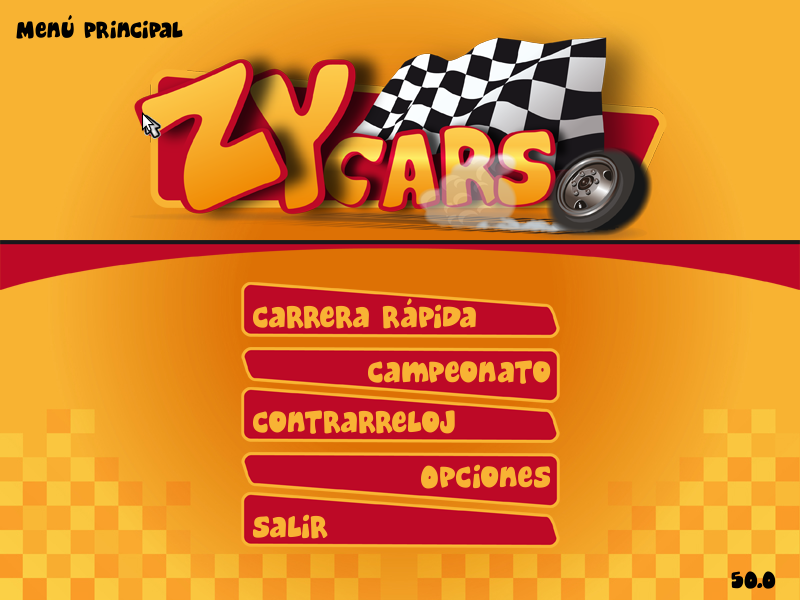
\includegraphics[scale=0.4]{imagenes/capturas/menuprincipal.png}
  \end{center}
  \caption{Manual de usuario: Menú principal}
\end{figure}

\paragraph{}
Debe usar el ratón para seleccionar la opción que desee.

%%%%%%%%%%%%%%%%%%%% MODOS DE JUEGO %%%%%%%%%%%%%%%%%%%%%%%
\section{Modos de juego}

\paragraph{}
En \emph{Zycars} hay disponibles tres modos de juegos, en los que competiremos solos o contra la máquina en función
del objetivo que tengamos que lograr.

\subsection{Carrera rápida}

\paragraph{}
El modo carrera rápida consiste en competir contra la inteligencia artificial en una única carrera, con el objetivo de 
mejorar nuestras habilidades y acostumbrarse a los controles del juego. A lo largo del circuito podremos obtener distintos
ítems con los que hacer frente a nuestros competidores.

\subsection{Campeonato}

\paragraph{}
En el modo Campeonato competiremos contra la inteligencia artificial a lo largo de cuatro circuitos, en los que obtendremos
una puntuación en relación a la posición que hayamos obtenido al concluir la carrera, 4 puntos para el ganador, 2 puntos para
el segundo clasificado, 1 punto para el tercero y 0 puntos para el ultimo en concluir la carrera. El competidor que más puntos haya 
conseguido al concluir el campeonato, será el ganador del mismo. En este modo
también encontraremos ítems durante las distintas carreras.

\subsection{Contrarreloj}

\paragraph{}
En este modo de juego, el modo contrarreloj, el objetivo será batir los
distintos récords de tiempo que tienen cada uno de los 
circuitos, podremos mejorar tanto el tiempo general de la carrera, como el tiempo obtenido en la vuelta más rápida. Tendremos
un máximo de 3 vueltas para mejorar los tiempos. En este modo de juego no
encontraremos ítems, ya que no tendremos ningún oponente
al que tengamos que batir.


%%%%%%%%%%%%%%%%%% SELECCION DE PERSONAJE %%%%%%%%%%%%%%%%%%%%
\section{Menú de selección de personaje}

\paragraph{}
Una vez seleccionado un modo de juego, pasaremos al menú de selección de personaje. En este menú se nos mostrarán todos
los personajes disponibles en \emph{Zycars}, así como el coche que cada uno de ellos conduce y las distintas características
que poseen los coches.

\begin{figure}[H]
  \label{menu_personaje}
  \begin{center}
    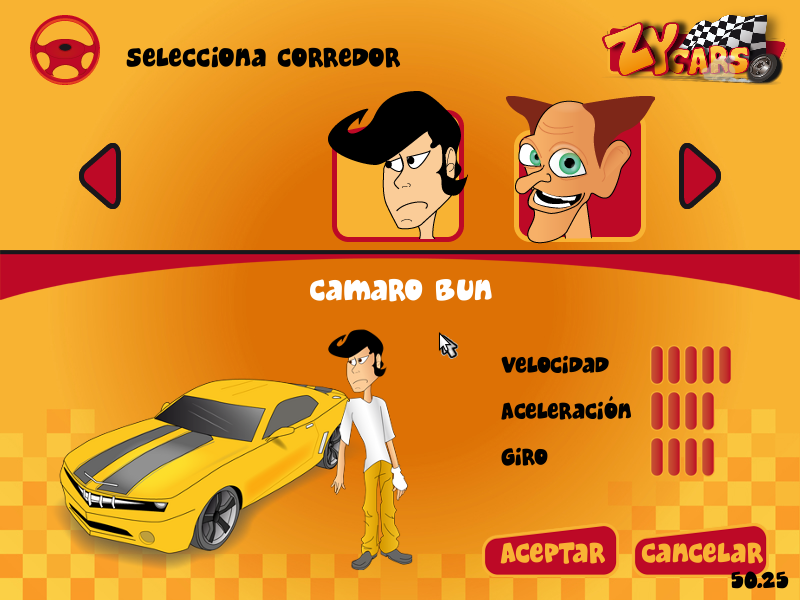
\includegraphics[scale=0.4]{imagenes/capturas/seleccionpersonaje.png}
  \end{center}
  \caption{Manual de usuario: Menú selección de personaje}
\end{figure}

\paragraph{}
Con el ratón podremos navegar sobre los distintos personajes pulsando sobre las flechas rojas. Pulsaremos en el botón
aceptar, para elegir el personaje seleccionado. Si queremos volver al menú principal, pulsaremos sobre el botón cancelar.

%%%%%%%%%%%%%%%%%% SELECCION DE CIRCUITO %%%%%%%%%%%%%%%%%%%%%
\section{Menú de selección de circuito}

\paragraph{}
Una vez seleccionado el personaje con el que deseamos competir, pasaremos al menú de selección de circuito. En este menú
se nos muestran los distintos campeonatos que posee el juego, así como los circuitos que componen cada uno de los 
campeonatos. 

\begin{figure}[H]
  \label{menu_circuito}
  \begin{center}
    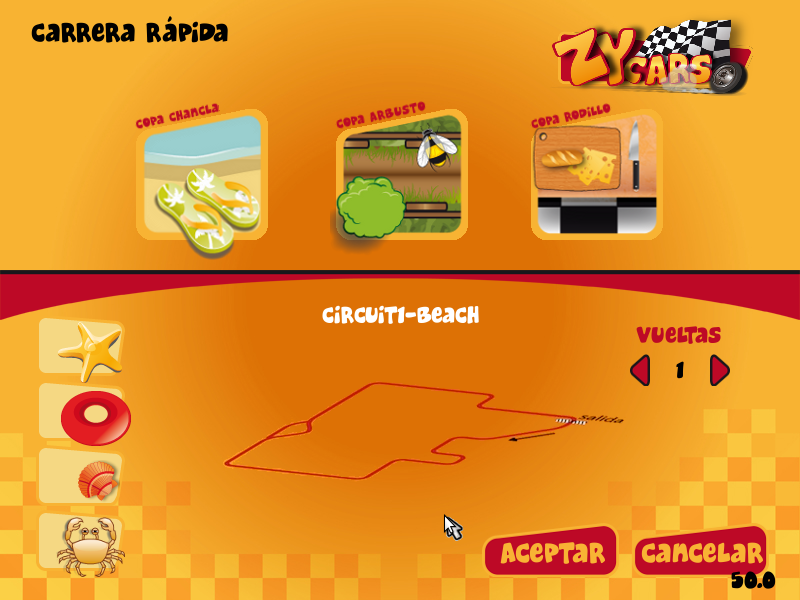
\includegraphics[scale=0.4]{imagenes/capturas/menucircuito.png}
  \end{center}
 \caption{Manual de usuario: Menú selección de circuito}
\end{figure}

\paragraph{}
Si nos encontramos en el modo carrera rápida o en el modo contrarreloj, deberemos seleccionar algún circuito de todos los
disponibles, una vez elegido, pulsaremos aceptar, en el caso de que queramos volver al menú de selección de personaje
pulsaremos sobre el botón cancelar.

\paragraph{}
Si estamos en el modo campeonato, podremos ver todos los circuitos que componen cada uno de los campeonato, al pulsar sobre
el botón aceptar, indicaremos que seleccionamos el campeonato actual. Si pulsamos el botón cancelar volveremos al menú de selección
de personaje.

\paragraph{}
Podremos elegir, en la parte derecha del menú, el número de vueltas que queremos que realicen en cada una de las carreras. Esta opción
no estará disponible en el modo campeonato, ya que en este modo siempre habrá que dar 3 vueltas al circuito.

%%%%%%%%%%%%%%%%%% OPCIONES %%%%%%%%%%%%%%%%%%%%%%
\section{Menú de Opciones}

\paragraph{}
En el menú de opciones, podremos modificar distintos apartados como sonido, características de pantalla y controles del juego. 
Una vez realizados los cambios y deseamos que se apliquen debemos pulsar el botón aceptar, si por el contrario deseamos volver al
menú principal si que se aplique ninguno de los cambios realizados, debemos pulsar sobre el botón cancelar.

\subsection{Sonido}

\paragraph{}
En este menú podremos seleccionar y modificar tanto el volumen de los efectos de sonido que se encuentran en el juego, así 
como el volumen de la música que escuchamos a lo largo de las distintas pantallas y circuitos.

\begin{figure}[H]
  \label{menu_audio}
  \begin{center}
    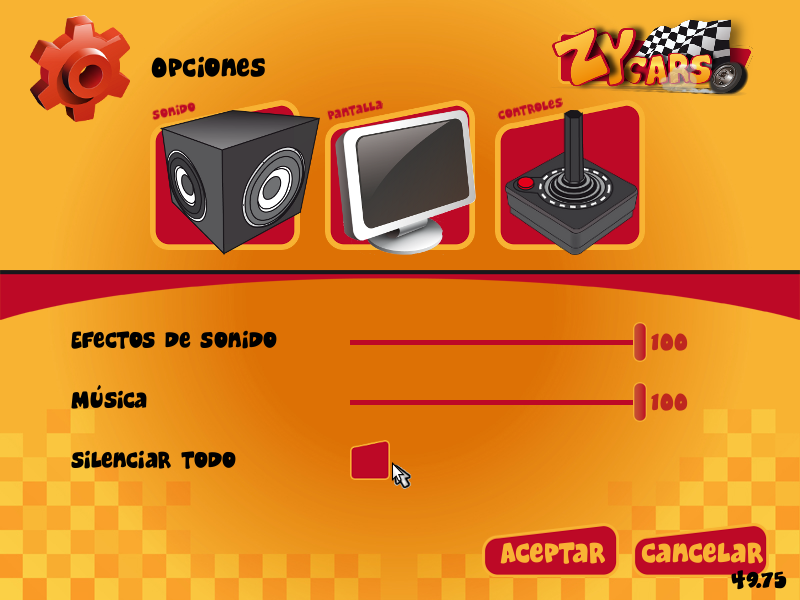
\includegraphics[scale=0.4]{imagenes/capturas/menuopcionesaudio.png}
  \end{center}
 \caption{Manual de usuario: Menú opciones - Audio}
\end{figure}

\paragraph{}
Como podemos ver, hay dos slider para la regulación del sonido y la música. También hay un checkbox, que nos permitirá silenciar todo, tanto 
los efectos de sonido como la música.

\subsection{Pantalla}

\paragraph{}
En este apartado solo dispondremos de una única opción. Esta opción nos
permitirá indicar si deseamos el juego a pantalla 
completa o si por el contrario lo deseamos al tamaño original de 800x600 píxeles.

\begin{figure}[H]
  \label{menu_pantalla}
  \begin{center}
    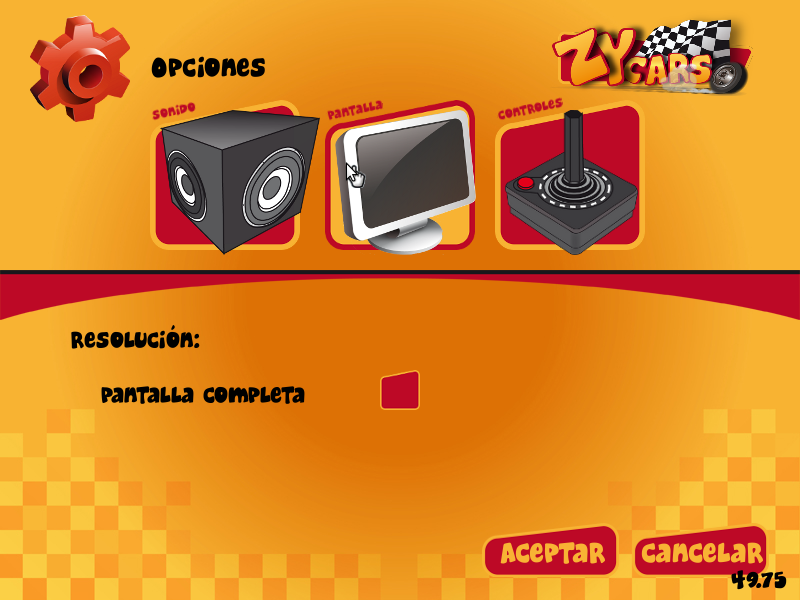
\includegraphics[scale=0.4]{imagenes/capturas/menuopcionespantalla.png}
  \end{center}
 \caption{Manual de usuario: Menú opciones - Pantalla}
\end{figure}

\subsection{Controles}

\paragraph{}
En esta sección del Menú de opciones podemos modificar que controles deseamos a la hora de manejar el vehículo. Los 
controles que podemos modificar son los de dirección, lanzamiento de los ítems y pausar el juego.

\begin{figure}[H]
  \label{menu_controles}
  \begin{center}
    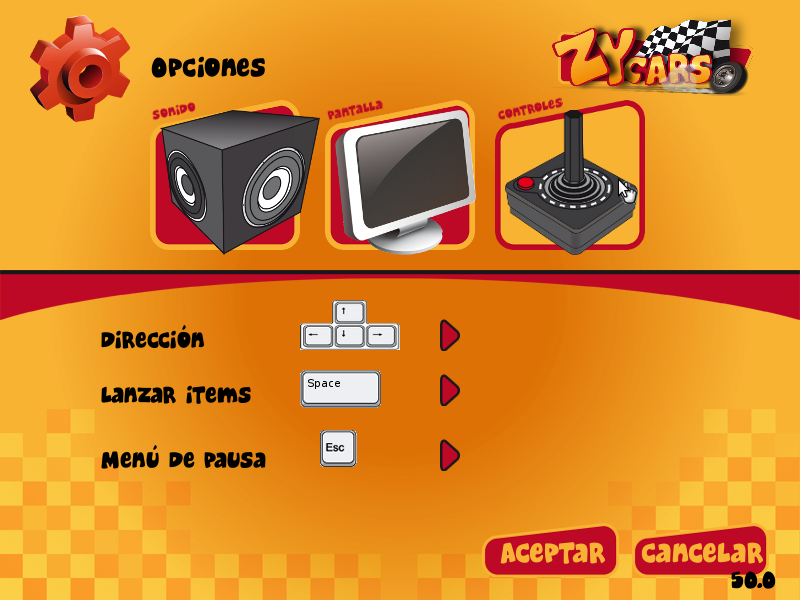
\includegraphics[scale=0.4]{imagenes/capturas/menuopcionescontroles.png}
  \end{center}
 \caption{Manual de usuario: Menú opciones - Controles}
\end{figure}

Debemos pulsar sobre las flechas para modificar los controles que queremos usar.

\section{Ítems}

\paragraph{}
Durante las carreras en las que compitamos contra la máquina, a lo largo de los circuitos encontraremos unas bolas que nos
proporcionarán distintos elementos con los que podremos atacar a nuestros oponentes, dejar obstáculos o aumenten nuestra velocidad
durante un periodo de tiempo.

\begin{figure}[H]
  \label{caja_item}
  \begin{center}
    
\includegraphics[scale=1]{imagenes/items/item_box.png}
  \end{center}
 \caption{Manual de usuario: Bola de ítem.}
\end{figure}

\paragraph{}
Los distintos ítem que podemos conseguir tras atravesar la bola de ítem se describen a continuación:

\begin{itemize}
    \item \textbf{Misil}: este ítem proporciona un único misil al jugador, el cual podremos lanzar a nuestros competidores,
    en caso de que el misil colisione con algún jugador, este perderá el control durante unos instantes. En el caso de que el 
    misil colisione con algún objeto colisionable explotará.
        \begin{figure}[H]
          \label{misil}
          \begin{center}
            
\includegraphics[scale=1]{imagenes/items/missile.png}
          \end{center}
         \caption{Manual de usuario: Misil.}
        \end{figure}
        
    \item \textbf{Misil x 3}: este ítem nos proporciona 3 misiles que tienen las mismas características que el misil normal, 
    introducido anteriormente.
        \begin{figure}[H]
          \label{tres_misiles}
          \begin{center}
            
\includegraphics[scale=1]{imagenes/items/3missile.png}
          \end{center}
         \caption{Manual de usuario: Tres misiles.}
        \end{figure}
        
    \item \textbf{Bola}: este ítem tiene las mismas características que un misil, la única diferencia existente es que al 
    colisionar con algún objete no explotará, si no que rebotará. Sólo explotará en el caso de que colisione con algún
    jugador.        
        \begin{figure}[H]
          \label{bola}
          \begin{center}
            
\includegraphics[scale=1]{imagenes/items/ball.png}
          \end{center}
         \caption{Manual de usuario: Bola.}
        \end{figure}
        
    \item \textbf{Chicle}: este ítem nos proporciona un chicle que al lanzarlo en el circuito, se pegará al asfalto de forma 
    permanente. Cualquier jugador que pase por encima de él, decrementará su velocidad.
        \begin{figure}[H]
          \label{chicle}
          \begin{center}
            
\includegraphics[scale=1]{imagenes/items/gum.png}
          \end{center}
         \caption{Manual de usuario: Chicle.}
        \end{figure}
        
    \item \textbf{Mancha de aceite}: este ítem nos proporciona una mancha de aceite que al lanzarla quedará en el circuito y 
    cualquier jugador que pase por encima, perderá el control del vehículo durante unos instantes.
        \begin{figure}[H]
          \label{mancha_aceite}
          \begin{center}
            
\includegraphics[scale=1]{imagenes/items/oil.png}
          \end{center}
         \caption{Manual de usuario: Macha de aceite.}
        \end{figure}
    
    \item \textbf{Turbo}: este ítem nos permitirá doblar nuestra velocidad durante unos instantes.
        \begin{figure}[H]
          \label{turbo}
          \begin{center}
            \includegraphics[scale=1]{imagenes/items/turbo.png}
          \end{center}
         \caption{Manual de usuario: Turbo.}
        \end{figure}
        
\end{itemize}



%\blackmatter
%\clearpage

\addcontentsline{toc}{chapter}{Bibliografia y referencias}
\begin{frame}
    \frametitle{Bibliografía recomendada}
    \begin{thebibliography}{5}
        \beamertemplatearticlebibitems
            \bibitem{Python}	
            Página de \emph{Python}
            \newblock http://www.python.org/
            
            \bibitem{PyGTK}
            Página oficial sobre \emph{Pygame}
            \newblock http://www.pygame.org/
             
        \beamertemplatebookbibitems
            \bibitem{UML}
            Larman, Craig
            \newblock Applying UML and Patterns, 3ª Edición. Prentice Hall, 2004.
            
            \bibitem{Dive into Python}
            Pilgrim, Mark
            \newblock Dive into Python. Appress, 2004.
    \end{thebibliography}
\end{frame}

\begin{frame}
    \frametitle{Demostración}
    
    \begin{center}
        {\Huge Demostración de Zycars}
    \end{center}
    
    \begin{center}
        \includegraphics[scale=0.25]{imagenes/logo_zycars.png}
    \end{center}

\end{frame}

\begin{frame}
    \frametitle{Esto es todo}
    
    \begin{center}
        {\Huge Gracias por su atención}\\
        \bigskip
        {\huge ¿Preguntas?}\\
        \bigskip
        {\LARGE http://code.google.com/p/zycars/}
    \end{center}

\end{frame}


\clearpage
% This is set up to run with pdflatex.
%---------The file header---------------------------------------------
%---------------------------------------------------------------------
\chapter*{\rlap{GNU Free Documentation License}}
\phantomsection  % so hyperref creates bookmarks
\addcontentsline{toc}{chapter}{GNU Free Documentation License}
%\label{label_fdl}

 \begin{center}

       Version 1.3, 3 November 2008


 Copyright \copyright{} 2000, 2001, 2002, 2007, 2008  Free Software Foundation, Inc.
 
 \bigskip
 
     <http://fsf.org/>
  
 \bigskip
 
 Everyone is permitted to copy and distribute verbatim copies
 of this license document, but changing it is not allowed.
\end{center}


\begin{center}
{\bf\large Preamble}
\end{center}

The purpose of this License is to make a manual, textbook, or other
functional and useful document ``free'' in the sense of freedom: to
assure everyone the effective freedom to copy and redistribute it,
with or without modifying it, either commercially or noncommercially.
Secondarily, this License preserves for the author and publisher a way
to get credit for their work, while not being considered responsible
for modifications made by others.

This License is a kind of ``copyleft'', which means that derivative
works of the document must themselves be free in the same sense.  It
complements the GNU General Public License, which is a copyleft
license designed for free software.

We have designed this License in order to use it for manuals for free
software, because free software needs free documentation: a free
program should come with manuals providing the same freedoms that the
software does.  But this License is not limited to software manuals;
it can be used for any textual work, regardless of subject matter or
whether it is published as a printed book.  We recommend this License
principally for works whose purpose is instruction or reference.


\begin{center}
{\Large\bf 1. APPLICABILITY AND DEFINITIONS\par}
\phantomsection
\addcontentsline{toc}{section}{1. APPLICABILITY AND DEFINITIONS}
\end{center}

This License applies to any manual or other work, in any medium, that
contains a notice placed by the copyright holder saying it can be
distributed under the terms of this License.  Such a notice grants a
world-wide, royalty-free license, unlimited in duration, to use that
work under the conditions stated herein.  The ``\textbf{Document}'', below,
refers to any such manual or work.  Any member of the public is a
licensee, and is addressed as ``\textbf{you}''.  You accept the license if you
copy, modify or distribute the work in a way requiring permission
under copyright law.

A ``\textbf{Modified Version}'' of the Document means any work containing the
Document or a portion of it, either copied verbatim, or with
modifications and/or translated into another language.

A ``\textbf{Secondary Section}'' is a named appendix or a front-matter section of
the Document that deals exclusively with the relationship of the
publishers or authors of the Document to the Document's overall subject
(or to related matters) and contains nothing that could fall directly
within that overall subject.  (Thus, if the Document is in part a
textbook of mathematics, a Secondary Section may not explain any
mathematics.)  The relationship could be a matter of historical
connection with the subject or with related matters, or of legal,
commercial, philosophical, ethical or political position regarding
them.

The ``\textbf{Invariant Sections}'' are certain Secondary Sections whose titles
are designated, as being those of Invariant Sections, in the notice
that says that the Document is released under this License.  If a
section does not fit the above definition of Secondary then it is not
allowed to be designated as Invariant.  The Document may contain zero
Invariant Sections.  If the Document does not identify any Invariant
Sections then there are none.

The ``\textbf{Cover Texts}'' are certain short passages of text that are listed,
as Front-Cover Texts or Back-Cover Texts, in the notice that says that
the Document is released under this License.  A Front-Cover Text may
be at most 5 words, and a Back-Cover Text may be at most 25 words.

A ``\textbf{Transparent}'' copy of the Document means a machine-readable copy,
represented in a format whose specification is available to the
general public, that is suitable for revising the document
straightforwardly with generic text editors or (for images composed of
pixels) generic paint programs or (for drawings) some widely available
drawing editor, and that is suitable for input to text formatters or
for automatic translation to a variety of formats suitable for input
to text formatters.  A copy made in an otherwise Transparent file
format whose markup, or absence of markup, has been arranged to thwart
or discourage subsequent modification by readers is not Transparent.
An image format is not Transparent if used for any substantial amount
of text.  A copy that is not ``Transparent'' is called ``\textbf{Opaque}''.

Examples of suitable formats for Transparent copies include plain
ASCII without markup, Texinfo input format, LaTeX input format, SGML
or XML using a publicly available DTD, and standard-conforming simple
HTML, PostScript or PDF designed for human modification.  Examples of
transparent image formats include PNG, XCF and JPG.  Opaque formats
include proprietary formats that can be read and edited only by
proprietary word processors, SGML or XML for which the DTD and/or
processing tools are not generally available, and the
machine-generated HTML, PostScript or PDF produced by some word
processors for output purposes only.

The ``\textbf{Title Page}'' means, for a printed book, the title page itself,
plus such following pages as are needed to hold, legibly, the material
this License requires to appear in the title page.  For works in
formats which do not have any title page as such, ``Title Page'' means
the text near the most prominent appearance of the work's title,
preceding the beginning of the body of the text.

The ``\textbf{publisher}'' means any person or entity that distributes
copies of the Document to the public.

A section ``\textbf{Entitled XYZ}'' means a named subunit of the Document whose
title either is precisely XYZ or contains XYZ in parentheses following
text that translates XYZ in another language.  (Here XYZ stands for a
specific section name mentioned below, such as ``\textbf{Acknowledgements}'',
``\textbf{Dedications}'', ``\textbf{Endorsements}'', or ``\textbf{History}''.)  
To ``\textbf{Preserve the Title}''
of such a section when you modify the Document means that it remains a
section ``Entitled XYZ'' according to this definition.

The Document may include Warranty Disclaimers next to the notice which
states that this License applies to the Document.  These Warranty
Disclaimers are considered to be included by reference in this
License, but only as regards disclaiming warranties: any other
implication that these Warranty Disclaimers may have is void and has
no effect on the meaning of this License.


\begin{center}
{\Large\bf 2. VERBATIM COPYING\par}
\phantomsection
\addcontentsline{toc}{section}{2. VERBATIM COPYING}
\end{center}

You may copy and distribute the Document in any medium, either
commercially or noncommercially, provided that this License, the
copyright notices, and the license notice saying this License applies
to the Document are reproduced in all copies, and that you add no other
conditions whatsoever to those of this License.  You may not use
technical measures to obstruct or control the reading or further
copying of the copies you make or distribute.  However, you may accept
compensation in exchange for copies.  If you distribute a large enough
number of copies you must also follow the conditions in section~3.

You may also lend copies, under the same conditions stated above, and
you may publicly display copies.


\begin{center}
{\Large\bf 3. COPYING IN QUANTITY\par}
\phantomsection
\addcontentsline{toc}{section}{3. COPYING IN QUANTITY}
\end{center}


If you publish printed copies (or copies in media that commonly have
printed covers) of the Document, numbering more than 100, and the
Document's license notice requires Cover Texts, you must enclose the
copies in covers that carry, clearly and legibly, all these Cover
Texts: Front-Cover Texts on the front cover, and Back-Cover Texts on
the back cover.  Both covers must also clearly and legibly identify
you as the publisher of these copies.  The front cover must present
the full title with all words of the title equally prominent and
visible.  You may add other material on the covers in addition.
Copying with changes limited to the covers, as long as they preserve
the title of the Document and satisfy these conditions, can be treated
as verbatim copying in other respects.

If the required texts for either cover are too voluminous to fit
legibly, you should put the first ones listed (as many as fit
reasonably) on the actual cover, and continue the rest onto adjacent
pages.

If you publish or distribute Opaque copies of the Document numbering
more than 100, you must either include a machine-readable Transparent
copy along with each Opaque copy, or state in or with each Opaque copy
a computer-network location from which the general network-using
public has access to download using public-standard network protocols
a complete Transparent copy of the Document, free of added material.
If you use the latter option, you must take reasonably prudent steps,
when you begin distribution of Opaque copies in quantity, to ensure
that this Transparent copy will remain thus accessible at the stated
location until at least one year after the last time you distribute an
Opaque copy (directly or through your agents or retailers) of that
edition to the public.

It is requested, but not required, that you contact the authors of the
Document well before redistributing any large number of copies, to give
them a chance to provide you with an updated version of the Document.


\begin{center}
{\Large\bf 4. MODIFICATIONS\par}
\phantomsection
\addcontentsline{toc}{section}{4. MODIFICATIONS}
\end{center}

You may copy and distribute a Modified Version of the Document under
the conditions of sections 2 and 3 above, provided that you release
the Modified Version under precisely this License, with the Modified
Version filling the role of the Document, thus licensing distribution
and modification of the Modified Version to whoever possesses a copy
of it.  In addition, you must do these things in the Modified Version:

\begin{itemize}
\item[A.] 
   Use in the Title Page (and on the covers, if any) a title distinct
   from that of the Document, and from those of previous versions
   (which should, if there were any, be listed in the History section
   of the Document).  You may use the same title as a previous version
   if the original publisher of that version gives permission.
   
\item[B.]
   List on the Title Page, as authors, one or more persons or entities
   responsible for authorship of the modifications in the Modified
   Version, together with at least five of the principal authors of the
   Document (all of its principal authors, if it has fewer than five),
   unless they release you from this requirement.
   
\item[C.]
   State on the Title page the name of the publisher of the
   Modified Version, as the publisher.
   
\item[D.]
   Preserve all the copyright notices of the Document.
   
\item[E.]
   Add an appropriate copyright notice for your modifications
   adjacent to the other copyright notices.
   
\item[F.]
   Include, immediately after the copyright notices, a license notice
   giving the public permission to use the Modified Version under the
   terms of this License, in the form shown in the Addendum below.
   
\item[G.]
   Preserve in that license notice the full lists of Invariant Sections
   and required Cover Texts given in the Document's license notice.
   
\item[H.]
   Include an unaltered copy of this License.
   
\item[I.]
   Preserve the section Entitled ``History'', Preserve its Title, and add
   to it an item stating at least the title, year, new authors, and
   publisher of the Modified Version as given on the Title Page.  If
   there is no section Entitled ``History'' in the Document, create one
   stating the title, year, authors, and publisher of the Document as
   given on its Title Page, then add an item describing the Modified
   Version as stated in the previous sentence.
   
\item[J.]
   Preserve the network location, if any, given in the Document for
   public access to a Transparent copy of the Document, and likewise
   the network locations given in the Document for previous versions
   it was based on.  These may be placed in the ``History'' section.
   You may omit a network location for a work that was published at
   least four years before the Document itself, or if the original
   publisher of the version it refers to gives permission.
   
\item[K.]
   For any section Entitled ``Acknowledgements'' or ``Dedications'',
   Preserve the Title of the section, and preserve in the section all
   the substance and tone of each of the contributor acknowledgements
   and/or dedications given therein.
   
\item[L.]
   Preserve all the Invariant Sections of the Document,
   unaltered in their text and in their titles.  Section numbers
   or the equivalent are not considered part of the section titles.
   
\item[M.]
   Delete any section Entitled ``Endorsements''.  Such a section
   may not be included in the Modified Version.
   
\item[N.]
   Do not retitle any existing section to be Entitled ``Endorsements''
   or to conflict in title with any Invariant Section.
   
\item[O.]
   Preserve any Warranty Disclaimers.
\end{itemize}

If the Modified Version includes new front-matter sections or
appendices that qualify as Secondary Sections and contain no material
copied from the Document, you may at your option designate some or all
of these sections as invariant.  To do this, add their titles to the
list of Invariant Sections in the Modified Version's license notice.
These titles must be distinct from any other section titles.

You may add a section Entitled ``Endorsements'', provided it contains
nothing but endorsements of your Modified Version by various
parties---for example, statements of peer review or that the text has
been approved by an organization as the authoritative definition of a
standard.

You may add a passage of up to five words as a Front-Cover Text, and a
passage of up to 25 words as a Back-Cover Text, to the end of the list
of Cover Texts in the Modified Version.  Only one passage of
Front-Cover Text and one of Back-Cover Text may be added by (or
through arrangements made by) any one entity.  If the Document already
includes a cover text for the same cover, previously added by you or
by arrangement made by the same entity you are acting on behalf of,
you may not add another; but you may replace the old one, on explicit
permission from the previous publisher that added the old one.

The author(s) and publisher(s) of the Document do not by this License
give permission to use their names for publicity for or to assert or
imply endorsement of any Modified Version.


\begin{center}
{\Large\bf 5. COMBINING DOCUMENTS\par}
\phantomsection
\addcontentsline{toc}{section}{5. COMBINING DOCUMENTS}
\end{center}


You may combine the Document with other documents released under this
License, under the terms defined in section~4 above for modified
versions, provided that you include in the combination all of the
Invariant Sections of all of the original documents, unmodified, and
list them all as Invariant Sections of your combined work in its
license notice, and that you preserve all their Warranty Disclaimers.

The combined work need only contain one copy of this License, and
multiple identical Invariant Sections may be replaced with a single
copy.  If there are multiple Invariant Sections with the same name but
different contents, make the title of each such section unique by
adding at the end of it, in parentheses, the name of the original
author or publisher of that section if known, or else a unique number.
Make the same adjustment to the section titles in the list of
Invariant Sections in the license notice of the combined work.

In the combination, you must combine any sections Entitled ``History''
in the various original documents, forming one section Entitled
``History''; likewise combine any sections Entitled ``Acknowledgements'',
and any sections Entitled ``Dedications''.  You must delete all sections
Entitled ``Endorsements''.

\begin{center}
{\Large\bf 6. COLLECTIONS OF DOCUMENTS\par}
\phantomsection
\addcontentsline{toc}{section}{6. COLLECTIONS OF DOCUMENTS}
\end{center}

You may make a collection consisting of the Document and other documents
released under this License, and replace the individual copies of this
License in the various documents with a single copy that is included in
the collection, provided that you follow the rules of this License for
verbatim copying of each of the documents in all other respects.

You may extract a single document from such a collection, and distribute
it individually under this License, provided you insert a copy of this
License into the extracted document, and follow this License in all
other respects regarding verbatim copying of that document.


\begin{center}
{\Large\bf 7. AGGREGATION WITH INDEPENDENT WORKS\par}
\phantomsection
\addcontentsline{toc}{section}{7. AGGREGATION WITH INDEPENDENT WORKS}
\end{center}


A compilation of the Document or its derivatives with other separate
and independent documents or works, in or on a volume of a storage or
distribution medium, is called an ``aggregate'' if the copyright
resulting from the compilation is not used to limit the legal rights
of the compilation's users beyond what the individual works permit.
When the Document is included in an aggregate, this License does not
apply to the other works in the aggregate which are not themselves
derivative works of the Document.

If the Cover Text requirement of section~3 is applicable to these
copies of the Document, then if the Document is less than one half of
the entire aggregate, the Document's Cover Texts may be placed on
covers that bracket the Document within the aggregate, or the
electronic equivalent of covers if the Document is in electronic form.
Otherwise they must appear on printed covers that bracket the whole
aggregate.


\begin{center}
{\Large\bf 8. TRANSLATION\par}
\phantomsection
\addcontentsline{toc}{section}{8. TRANSLATION}
\end{center}


Translation is considered a kind of modification, so you may
distribute translations of the Document under the terms of section~4.
Replacing Invariant Sections with translations requires special
permission from their copyright holders, but you may include
translations of some or all Invariant Sections in addition to the
original versions of these Invariant Sections.  You may include a
translation of this License, and all the license notices in the
Document, and any Warranty Disclaimers, provided that you also include
the original English version of this License and the original versions
of those notices and disclaimers.  In case of a disagreement between
the translation and the original version of this License or a notice
or disclaimer, the original version will prevail.

If a section in the Document is Entitled ``Acknowledgements'',
``Dedications'', or ``History'', the requirement (section~4) to Preserve
its Title (section~1) will typically require changing the actual
title.


\begin{center}
{\Large\bf 9. TERMINATION\par}
\phantomsection
\addcontentsline{toc}{section}{9. TERMINATION}
\end{center}


You may not copy, modify, sublicense, or distribute the Document
except as expressly provided under this License.  Any attempt
otherwise to copy, modify, sublicense, or distribute it is void, and
will automatically terminate your rights under this License.

However, if you cease all violation of this License, then your license
from a particular copyright holder is reinstated (a) provisionally,
unless and until the copyright holder explicitly and finally
terminates your license, and (b) permanently, if the copyright holder
fails to notify you of the violation by some reasonable means prior to
60 days after the cessation.

Moreover, your license from a particular copyright holder is
reinstated permanently if the copyright holder notifies you of the
violation by some reasonable means, this is the first time you have
received notice of violation of this License (for any work) from that
copyright holder, and you cure the violation prior to 30 days after
your receipt of the notice.

Termination of your rights under this section does not terminate the
licenses of parties who have received copies or rights from you under
this License.  If your rights have been terminated and not permanently
reinstated, receipt of a copy of some or all of the same material does
not give you any rights to use it.


\begin{center}
{\Large\bf 10. FUTURE REVISIONS OF THIS LICENSE\par}
\phantomsection
\addcontentsline{toc}{section}{10. FUTURE REVISIONS OF THIS LICENSE}
\end{center}


The Free Software Foundation may publish new, revised versions
of the GNU Free Documentation License from time to time.  Such new
versions will be similar in spirit to the present version, but may
differ in detail to address new problems or concerns.  See
http://www.gnu.org/copyleft/.

Each version of the License is given a distinguishing version number.
If the Document specifies that a particular numbered version of this
License ``or any later version'' applies to it, you have the option of
following the terms and conditions either of that specified version or
of any later version that has been published (not as a draft) by the
Free Software Foundation.  If the Document does not specify a version
number of this License, you may choose any version ever published (not
as a draft) by the Free Software Foundation.  If the Document
specifies that a proxy can decide which future versions of this
License can be used, that proxy's public statement of acceptance of a
version permanently authorizes you to choose that version for the
Document.


\begin{center}
{\Large\bf 11. RELICENSING\par}
\phantomsection
\addcontentsline{toc}{section}{11. RELICENSING}
\end{center}


``Massive Multiauthor Collaboration Site'' (or ``MMC Site'') means any
World Wide Web server that publishes copyrightable works and also
provides prominent facilities for anybody to edit those works.  A
public wiki that anybody can edit is an example of such a server.  A
``Massive Multiauthor Collaboration'' (or ``MMC'') contained in the
site means any set of copyrightable works thus published on the MMC
site.

``CC-BY-SA'' means the Creative Commons Attribution-Share Alike 3.0
license published by Creative Commons Corporation, a not-for-profit
corporation with a principal place of business in San Francisco,
California, as well as future copyleft versions of that license
published by that same organization.

``Incorporate'' means to publish or republish a Document, in whole or
in part, as part of another Document.

An MMC is ``eligible for relicensing'' if it is licensed under this
License, and if all works that were first published under this License
somewhere other than this MMC, and subsequently incorporated in whole
or in part into the MMC, (1) had no cover texts or invariant sections,
and (2) were thus incorporated prior to November 1, 2008.

The operator of an MMC Site may republish an MMC contained in the site
under CC-BY-SA on the same site at any time before August 1, 2009,
provided the MMC is eligible for relicensing.


\begin{center}
{\Large\bf ADDENDUM: How to use this License for your documents\par}
\phantomsection
\addcontentsline{toc}{section}{ADDENDUM: How to use this License for your documents}
\end{center}

To use this License in a document you have written, include a copy of
the License in the document and put the following copyright and
license notices just after the title page:

\bigskip
\begin{quote}
    Copyright \copyright{}  YEAR  YOUR NAME.
    Permission is granted to copy, distribute and/or modify this document
    under the terms of the GNU Free Documentation License, Version 1.3
    or any later version published by the Free Software Foundation;
    with no Invariant Sections, no Front-Cover Texts, and no Back-Cover Texts.
    A copy of the license is included in the section entitled ``GNU
    Free Documentation License''.
\end{quote}
\bigskip
    
If you have Invariant Sections, Front-Cover Texts and Back-Cover Texts,
replace the ``with \dots\ Texts.'' line with this:

\bigskip
\begin{quote}
    with the Invariant Sections being LIST THEIR TITLES, with the
    Front-Cover Texts being LIST, and with the Back-Cover Texts being LIST.
\end{quote}
\bigskip
    
If you have Invariant Sections without Cover Texts, or some other
combination of the three, merge those two alternatives to suit the
situation.

If your document contains nontrivial examples of program code, we
recommend releasing these examples in parallel under your choice of
free software license, such as the GNU General Public License,
to permit their use in free software.

%---------------------------------------------------------------------


\end{document}
